
\documentclass{book}
\usepackage[utf8]{inputenc}
\usepackage{graphicx}
\usepackage{tikz}
\usepackage{float}
\usepackage{wrapfig,lipsum}
\usepackage{svg}
\usepackage{mathtools}
\usepackage{tabu}
%\usepackage{subcaption}
\usepackage{subfigure}
\usepackage[a4paper, total={6in, 8in}]{geometry}

\definecolor{bg}{rgb}{0.95,0.95,0.95}




\begin{document}


\newcommand{\vecthreeBF}[1]{\vec{\textbf{#1}}}
\newcommand{\vecthree}[1]{\vec{#1}}
\newcommand{\vecNum}[3]{(#1, #2, #3)}

\newcommand{\parDeriv}[2]{\frac{\partial #1}{\partial #2}}
\newcommand{\parDerivS}[2]{\frac{\partial^2 #1}{\partial #2^2}}
\newcommand{\derivS}[2]{\frac{d^2 #1}{d#2^2}}

\newcommand{\dotProdBF}[2]{\vecthreeBF{#1} \cdot \vecthreeBF{#2}}
\newcommand{\dotProd}[2]{\vecthree{#1} \cdot \vecthree{#2}}

\newcommand{\crossProdBF}[2]{\vecthreeBF{#1} \times \vecthreeBF{#2}}
\newcommand{\crossProd}[2]{\vecthree{#1} \times \vecthree{#2}}

\newcommand{\e}{$\textbf{e}^-$ }
\newcommand{\egun}{$\textbf{e}^-$-gun }
\newcommand{\eB}{$\textbf{e}^-$ - $\vecthreeBF{B}$ }
\newcommand{\eE}{$\textbf{e}^-$ - $\vecthreeBF{E}$ }
\newcommand{\eEM}{$\textbf{e}^-$ - \textbf{EM} }
\newcommand{\ee}{$\textbf{e}^-$ - $\textbf{e}^-$ }


\newcommand{\fromeq}[1]{\textit{equation \ref{eq:#1}}}
\newcommand{\fromeqs}[2]{\textit{equations \ref{eq:#1} and \ref{eq:#2}}}
\newcommand{\fromeqsth}[3]{\textit{equations \ref{eq:#1}, \ref{eq:#2} and \ref{eq:#3}}}
\newcommand{\fromeqsf}[4]{\textit{equations \ref{eq:#1}, \ref{eq:#2}, \ref{eq:#3} and \ref{eq:#4}}}

\newcommand{\fromfig}[1]{\textit{figure \ref{fig:#1}}}
\newcommand{\fromfigs}[2]{\textit{figures \ref{fig:#1} and \ref{fig:#2}}}
\newcommand{\fromfigf}[4]{\textit{figures \ref{fig:#1}, \ref{fig:#2}, \ref{fig:#3} and \ref{fig:#4}}}

\newcommand{\fromsec}[1]{\textit{section \ref{sec:#1}}}
\newcommand{\fromsecs}[2]{\textit{sections \ref{sec:#1} and \ref{sec:#2}}}

\newcommand{\fromapp}[1]{\textit{Appendix \ref{appendix:#1}}}

\newcommand{\fromtab}[1]{\textit{Table \ref{tab:#1}}}
\newcommand{\fromtabs}[2]{\textit{Tables \ref{tab:#1} and \ref{tab:#2}}}


\newcommand{\comment}[1]{}



%----../../..++++.

%%%%%%
% Start of mani.tex
\section{Manifacturing}

Manifacturing of the rhodotron cavity has been ongoing, planned to be completed in the following months.

The cavity itself was manifactured as 5 main parts, using 5mm thick stainless steel sheet. 
Elastic version of the 304, 304L was chosen to be the production material for ease of bending.
These sheets were then pressed to achieve the shapes of the parts. 
Several flanges were then machined, including
\begin{itemize}
    \item $4.5$in EIA RF flange for RF input,
    \item ISO-100KF vacuum connector flanges for vacuum pumps,
    \item ISO-63 KF flange for probe insertion,
    \item KF-40 flanges for beam line vacuum gauges.
\end{itemize}
After desired shapes were produced inside surface of the sheets were polished with 2000 grits. 
304 stainless steel sheet bars of different sizes were then added by 
TIG welding to achieve pressure resistance.

Because the main body of the cavity was 5mm thick and 304L was used, deformations on cylinderical symmetry were encountered. 
This problem was solved by welding 6 10mm thick toroidal sheets between the coaxial cylinders, 
which would be removed after the heat treatment.
\iffalse \begin{figure}
    %\captionsetup[subfigure]{justification=centering}
    %\captionsetup{justification=centering}
    \centering
    \begin{subfigure}{.5\textwidth}
      \centering
      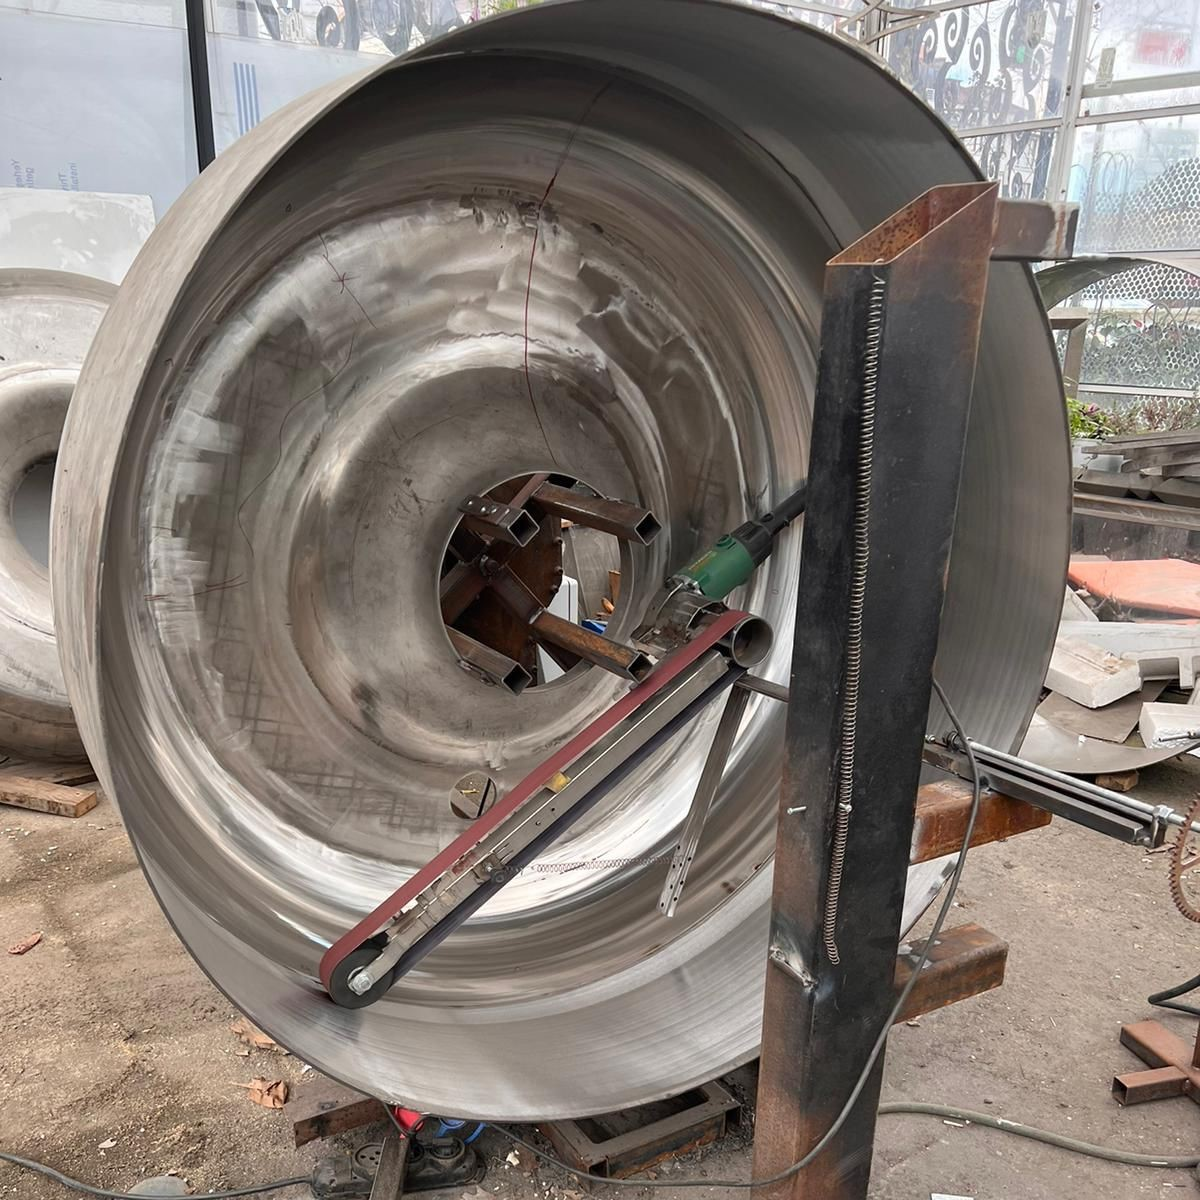
\includegraphics[width=.96\linewidth]{../../../figures/manif/polish/rhodo_bottom_unpolished_cropped.jpeg}
      \caption{Bottom part of the cavity while polishing.}
    \end{subfigure}%
    \centering
    \begin{subfigure}{.5\textwidth}
      \centering
      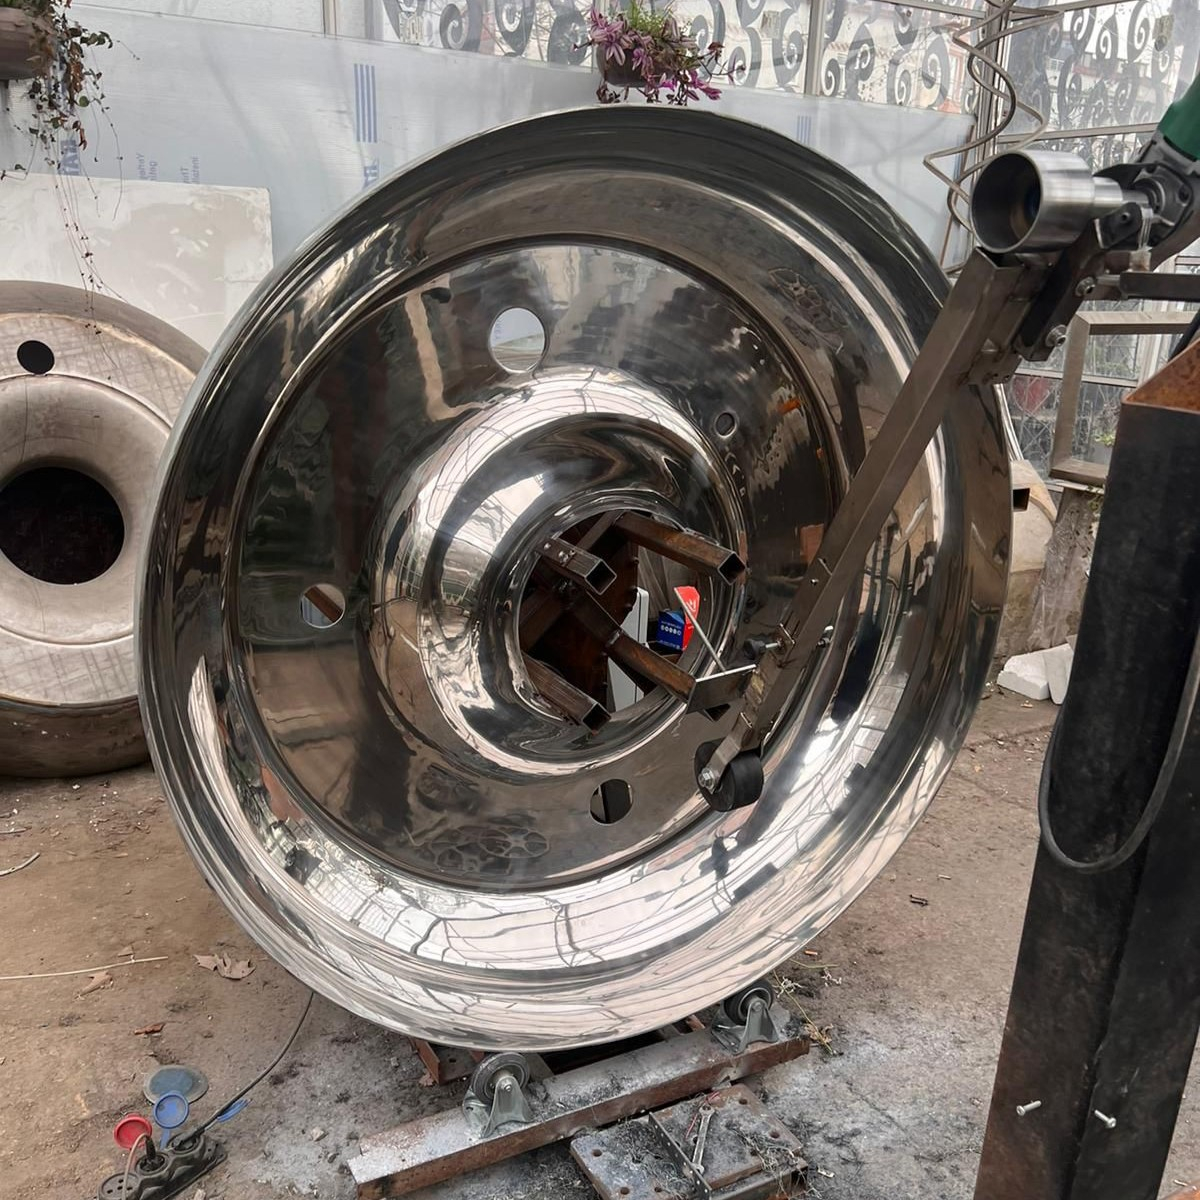
\includegraphics[width=.96\linewidth]{../../../figures/manif/polish/rhodo_upper_polished_cropped.jpeg}
      \caption{Top part of the cavity after polishing.}
    \end{subfigure}
    \caption{Polishing of the inner surface of cavity.}
    \label{fig:manif_polishing}
\end{figure} \fi

\begin{figure}[H]
    \centering
    \subfigure[\centering Bottom part of the cavity while polishing]{{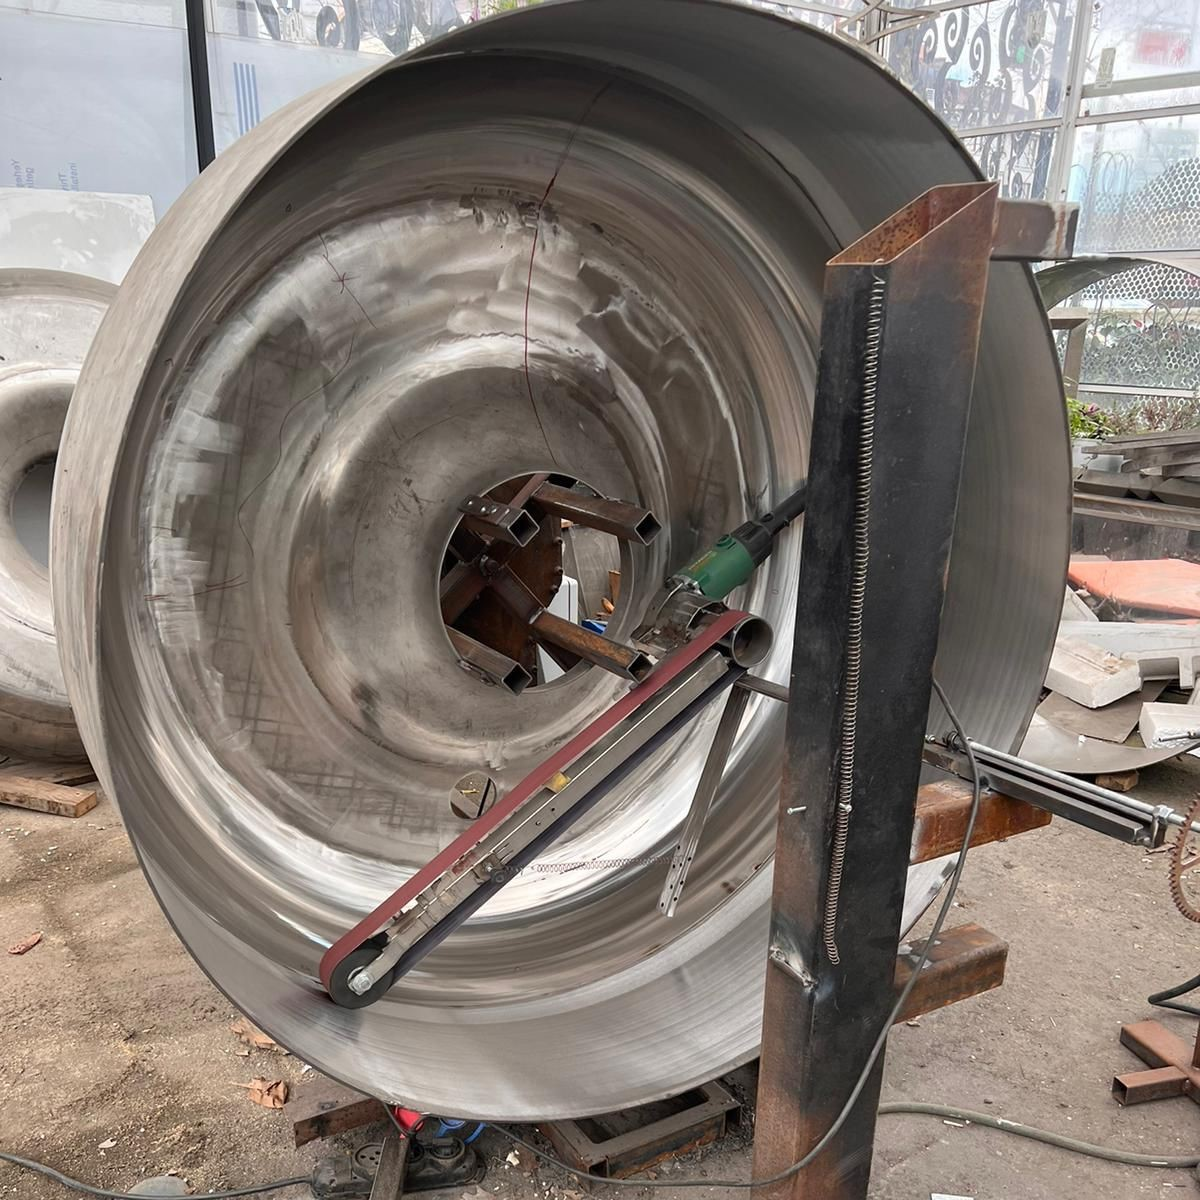
\includegraphics[width=.46\textwidth]{../../../figures/manif/polish/rhodo_bottom_unpolished_cropped.jpeg} }}%
    \qquad\subfigure[\centering Top part of the cavity after polishing]{{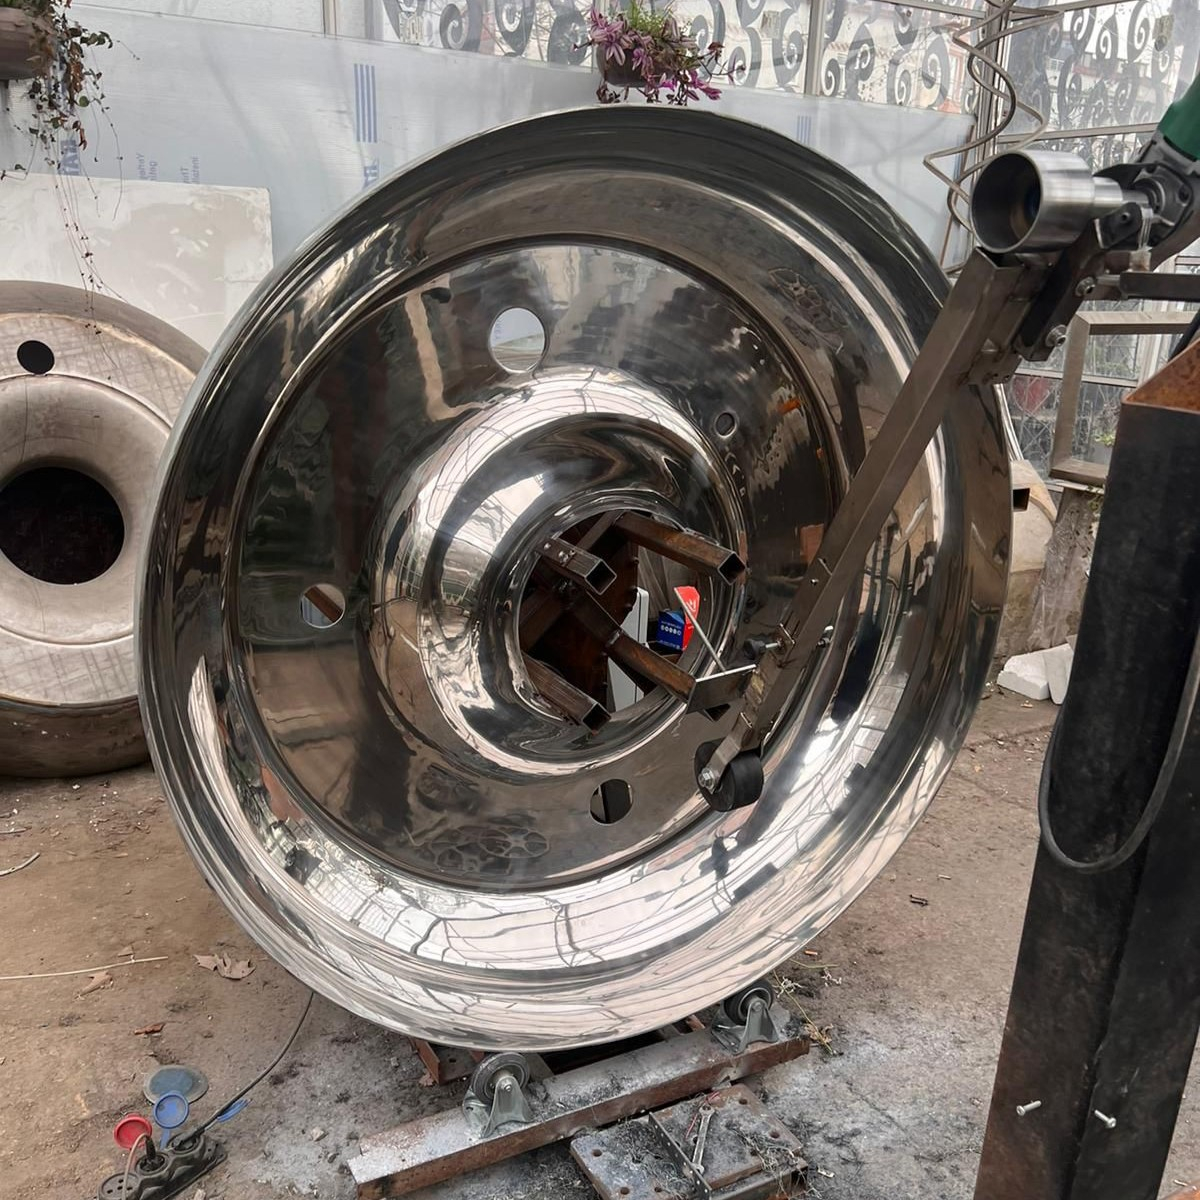
\includegraphics[width=.46\textwidth]{../../../figures/manif/polish/rhodo_upper_polished_cropped.jpeg} }}%
    \vspace{5pt}
    \caption{Polishing of the inner surface of cavity.}
    \label{fig:manif_polishing}
    \vspace{5pt}
\end{figure}

\iffalse \begin{figure}
    %\captionsetup[subfigure]{justification=centering}
    %\captionsetup{justification=centering}
    \centering
    \begin{subfigure}{.5\textwidth}
      \centering
      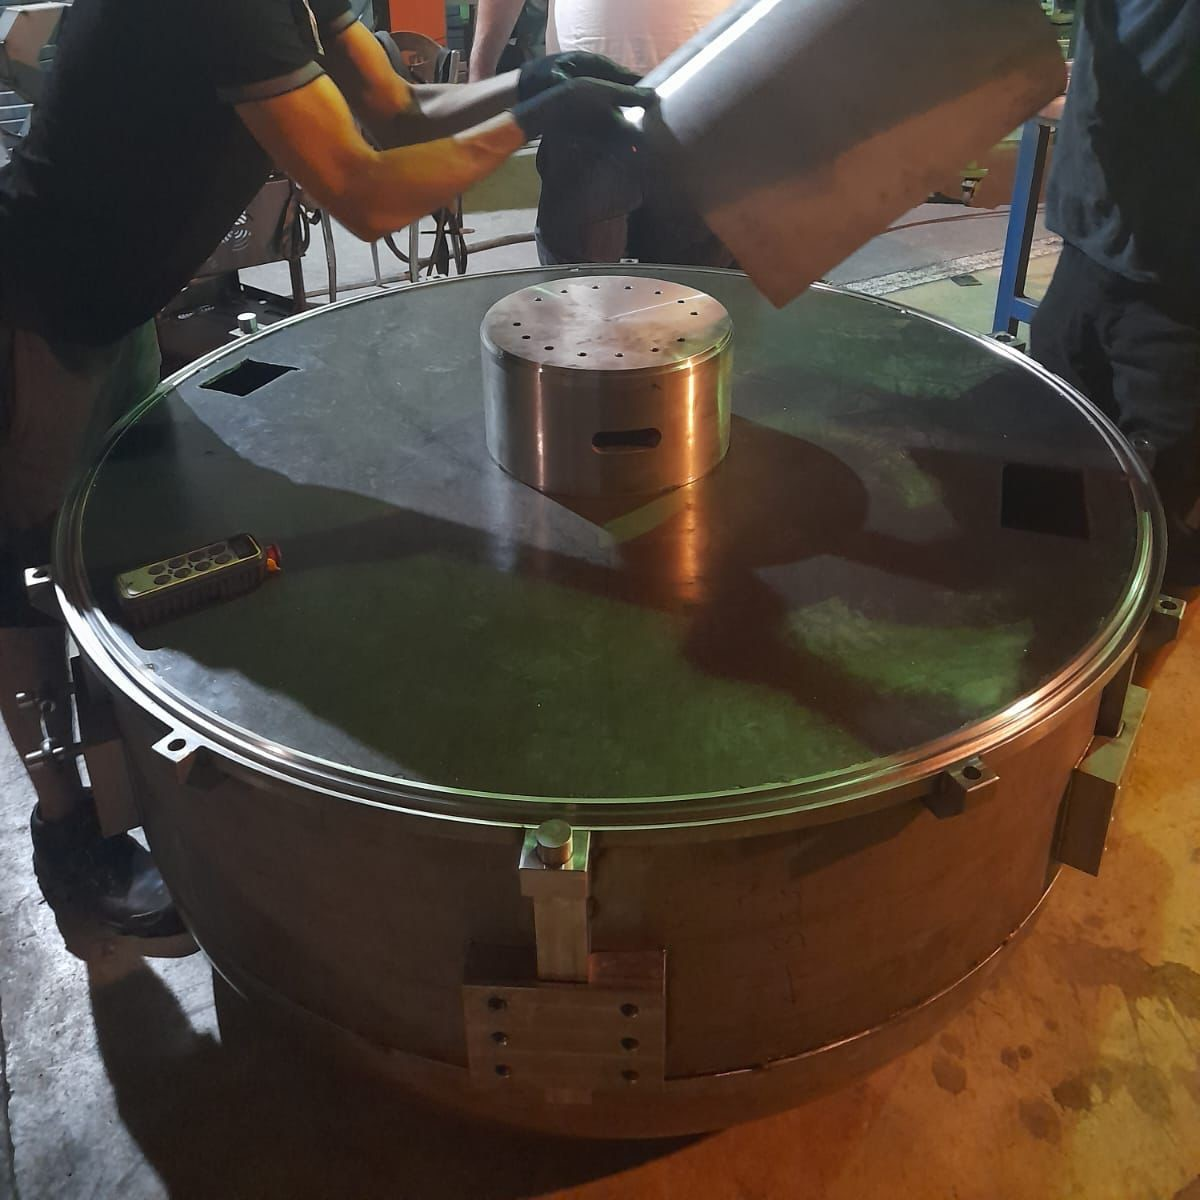
\includegraphics[width=.96\linewidth]{../../../figures/manif/toroidal_sheets/rhodo_bottom_cropped.jpeg}
      \caption{Bottom part of the cavity with the exposed beam line in inner cylinder.}
    \end{subfigure}%
    \centering
    \begin{subfigure}{.5\textwidth}
      \centering
      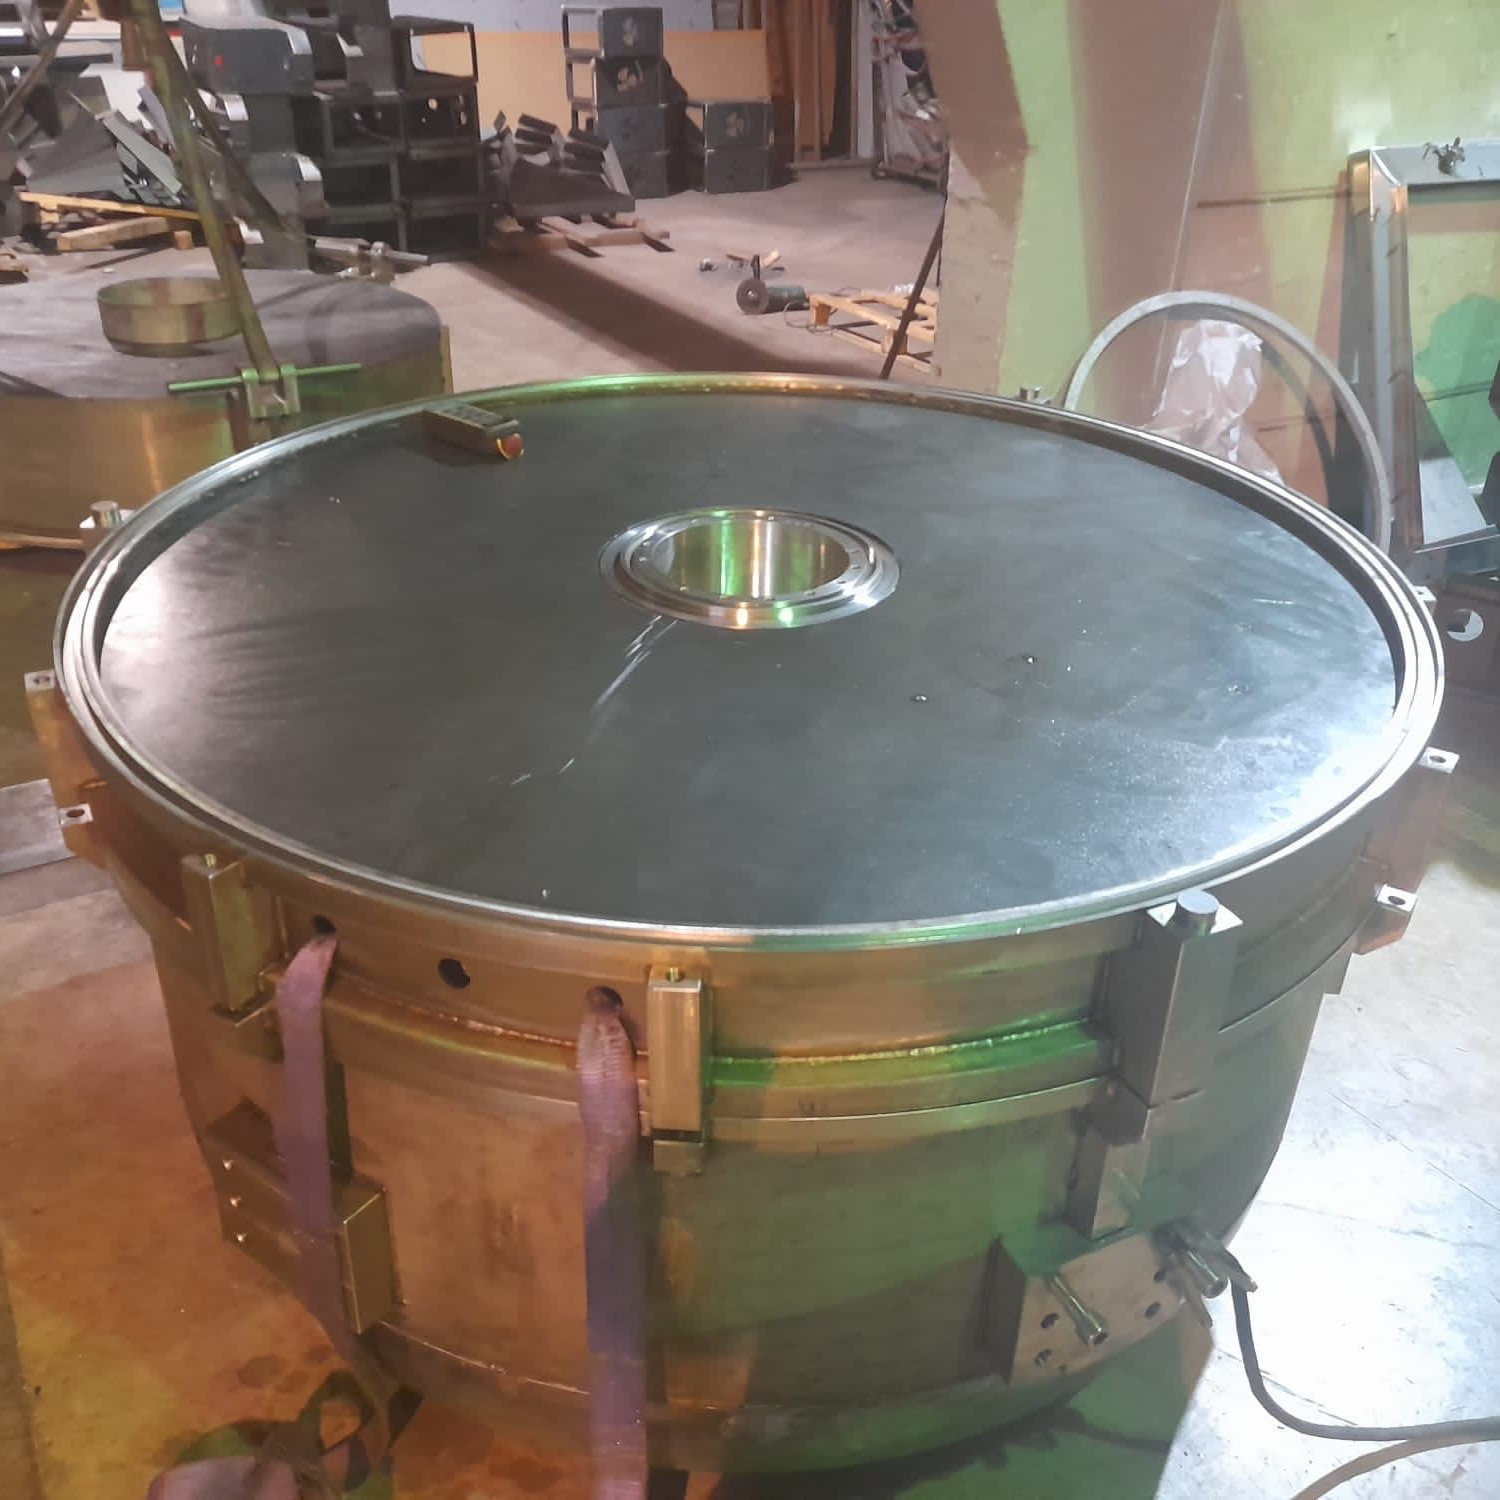
\includegraphics[width=.96\linewidth]{../../../figures/manif/toroidal_sheets/rhodo_middle_toroidal_sheets_welded_cropped.jpeg}
      \caption{Bottom part of the cavity with the beam line assembled.}
    \end{subfigure}
    \caption{Deformation prevention measure, 10 mm thick toroidal sheets.}
    \label{fig:manif_toroidal_sheets}
\end{figure} \fi
\begin{figure}[H]
    \centering
    \subfigure[\centering Bottom part of the cavity with the exposed beam line in inner cylinder]{{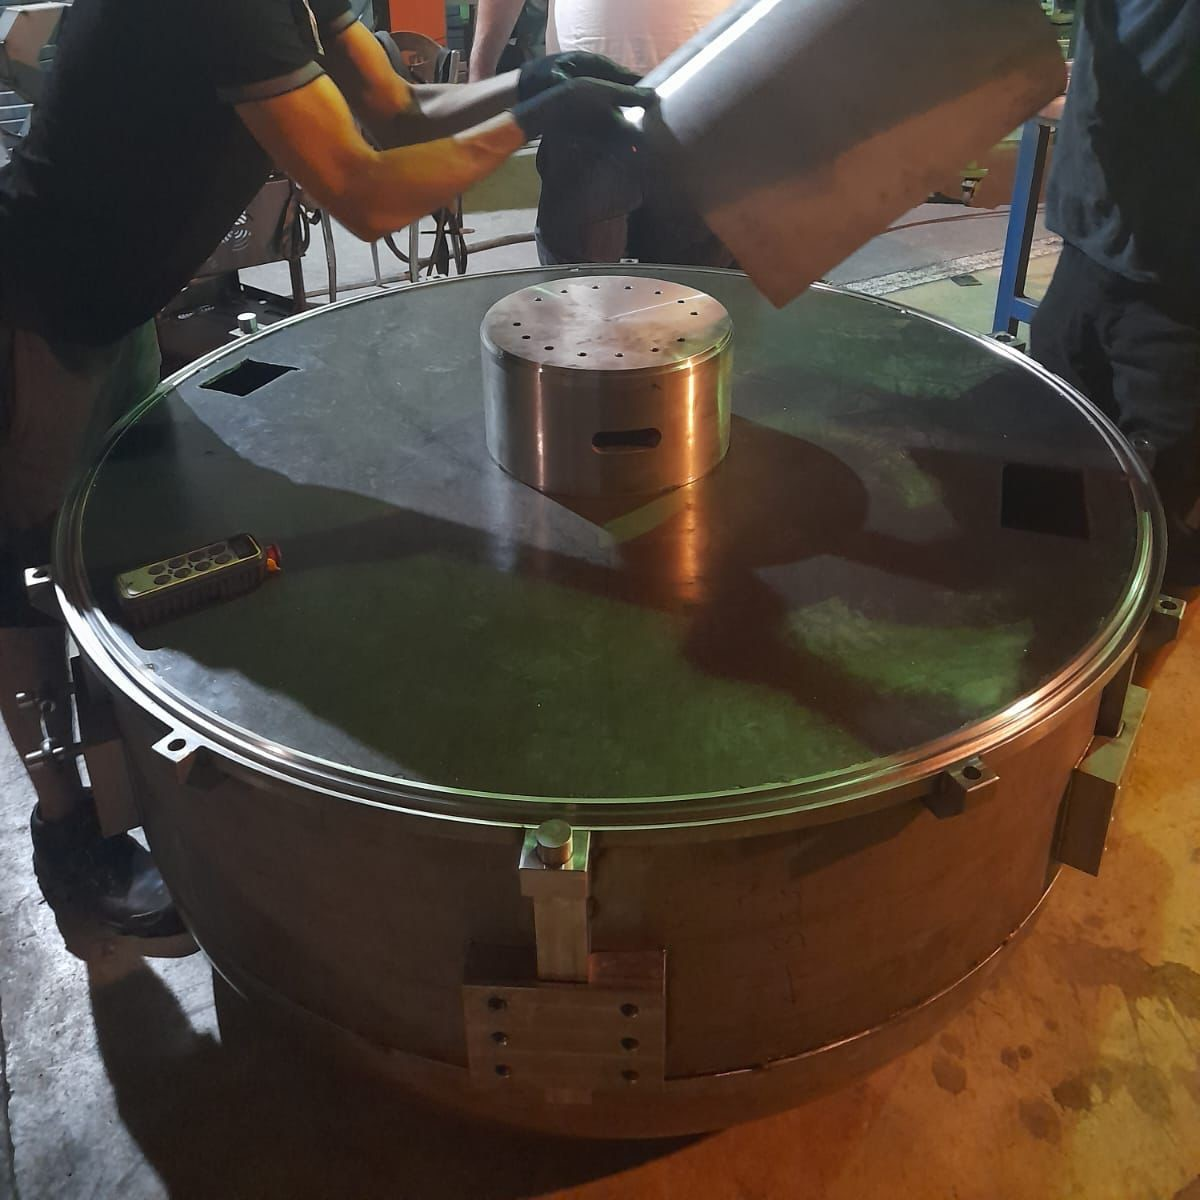
\includegraphics[width=.46\textwidth]{../../../figures/manif/toroidal_sheets/rhodo_bottom_cropped.jpeg} }}%
    \qquad\subfigure[\centering Bottom part of the cavity with the beam line assembled]{{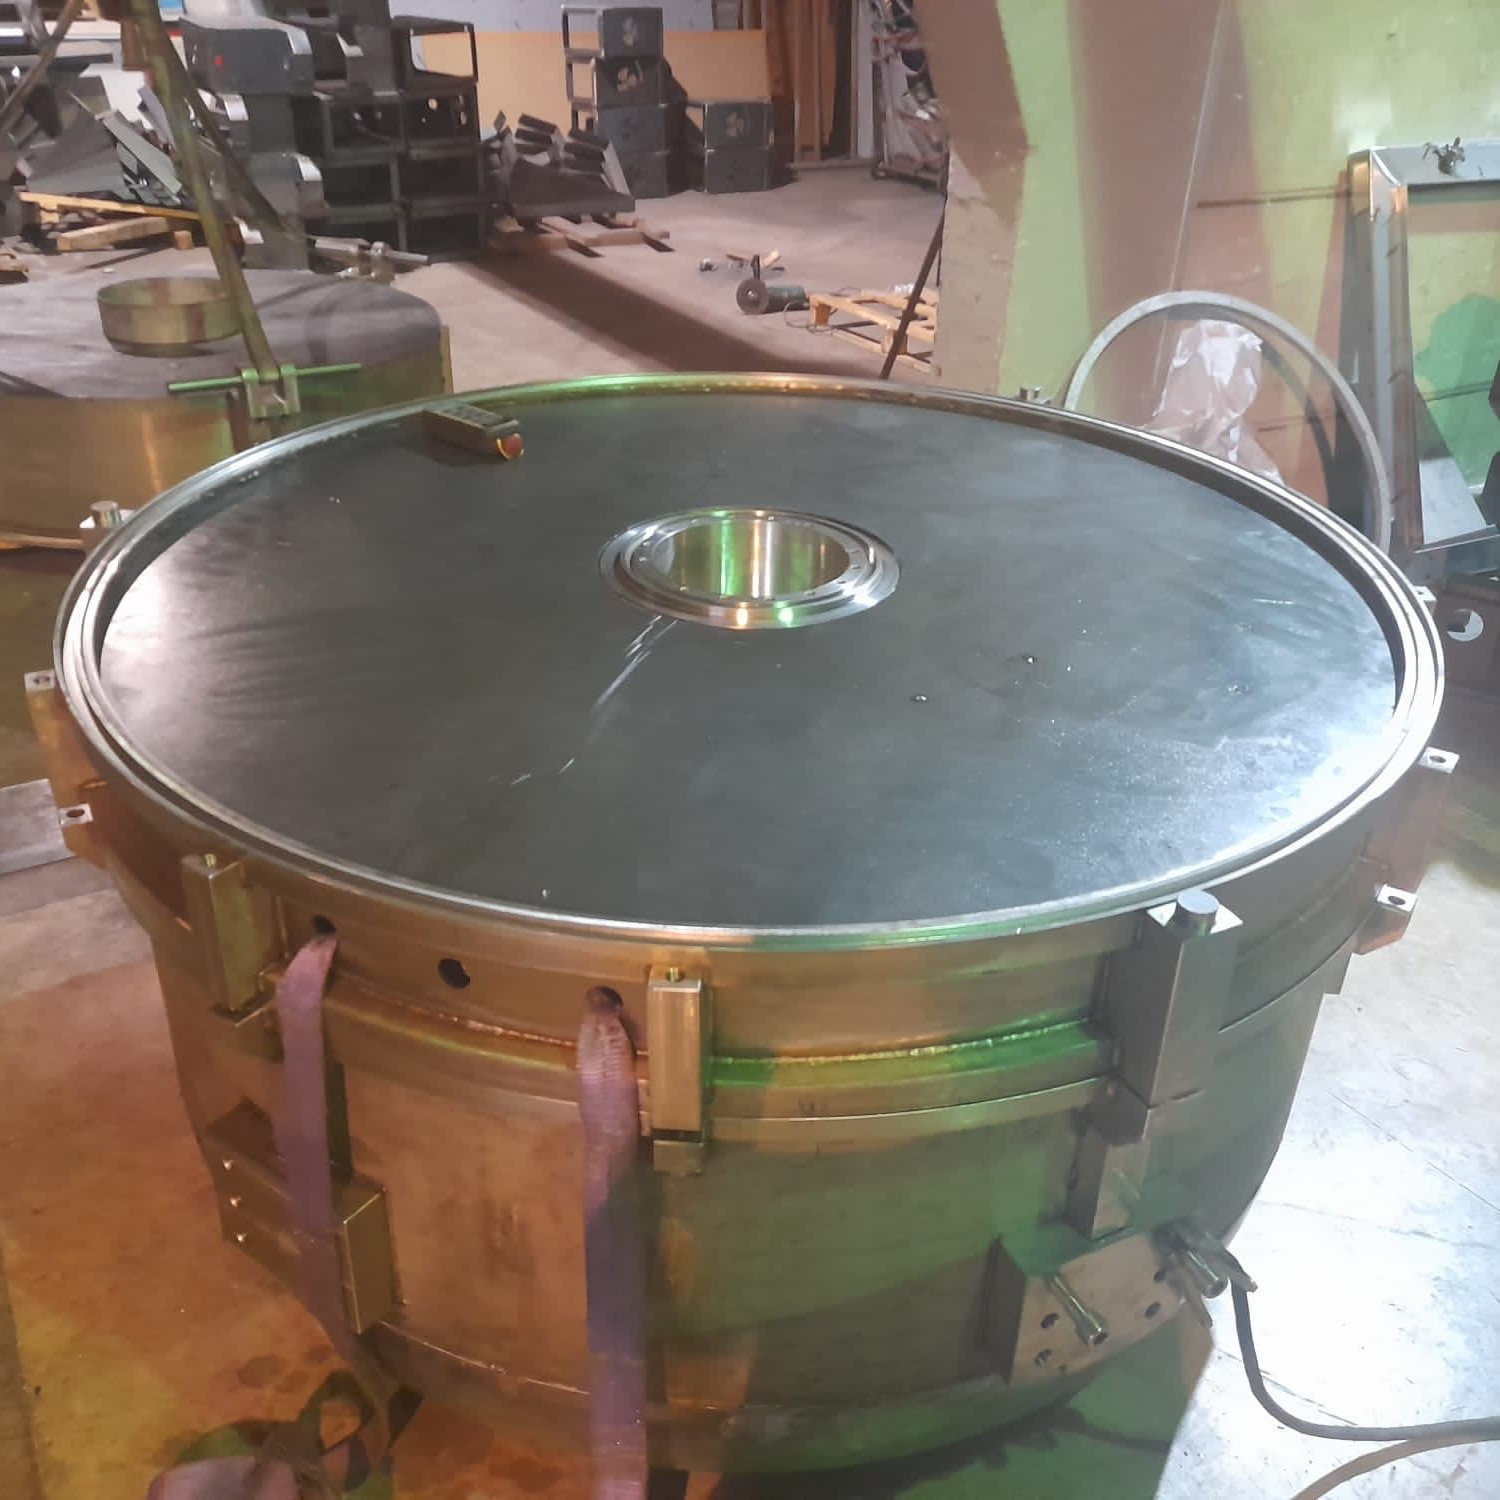
\includegraphics[width=.46\textwidth]{../../../figures/manif/toroidal_sheets/rhodo_middle_toroidal_sheets_welded_cropped.jpeg} }}%
    \vspace{5pt}
    \caption{Deformation prevention measure, 10 mm thick toroidal sheets.}
    \label{fig:manif_toroidal_sheets}
\end{figure}

\begin{figure}[H]
    %%\captionsetup{justification=centering}
    \centering
    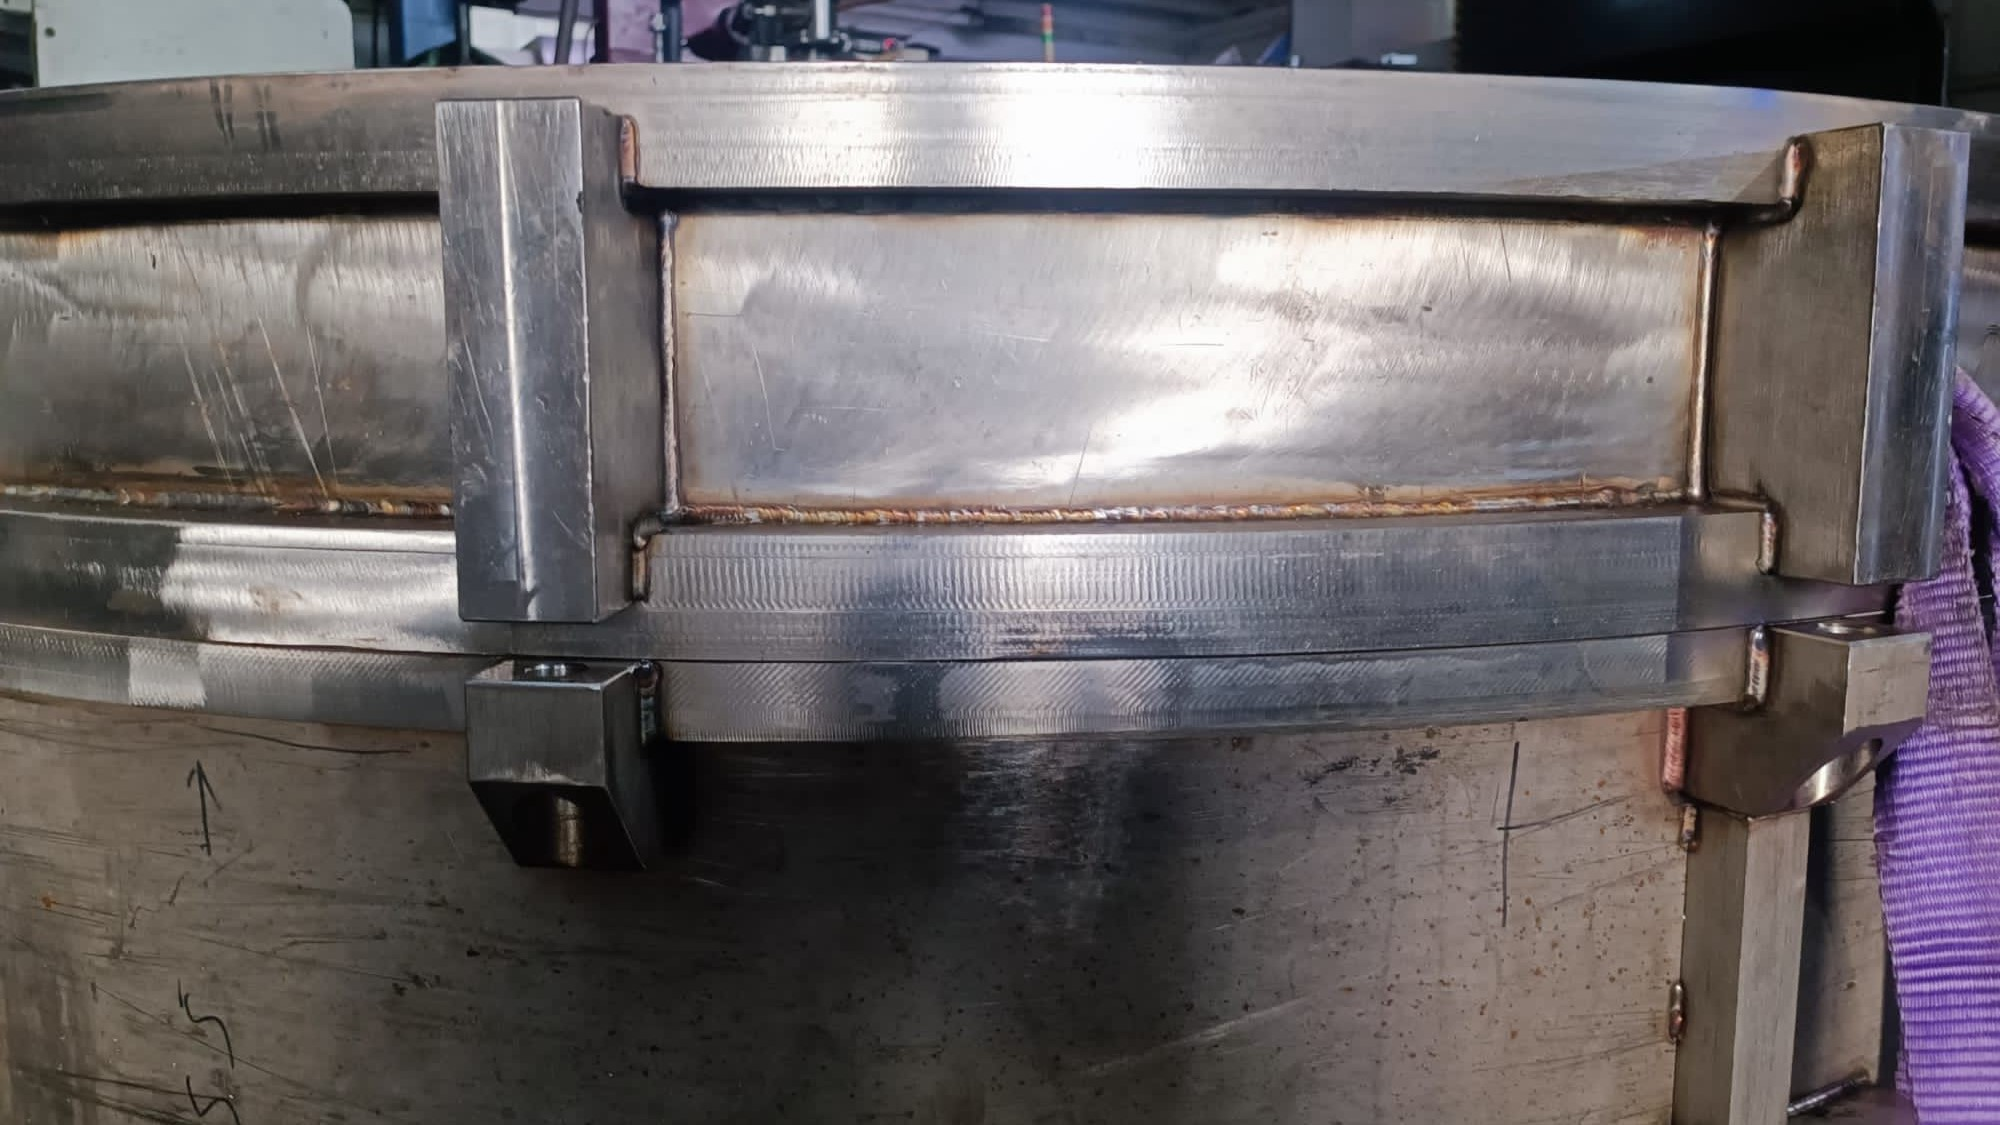
\includegraphics[width=.8\linewidth]{../../../figures/manif/welding/rhodo_middle_sheetbars_cropped.jpeg}
    \vspace{0pt}
    \caption{Welded sheet bars.}
    \vspace{5pt}
\end{figure}

\begin{figure}[H]
    %%\captionsetup{justification=centering}
    \centering
    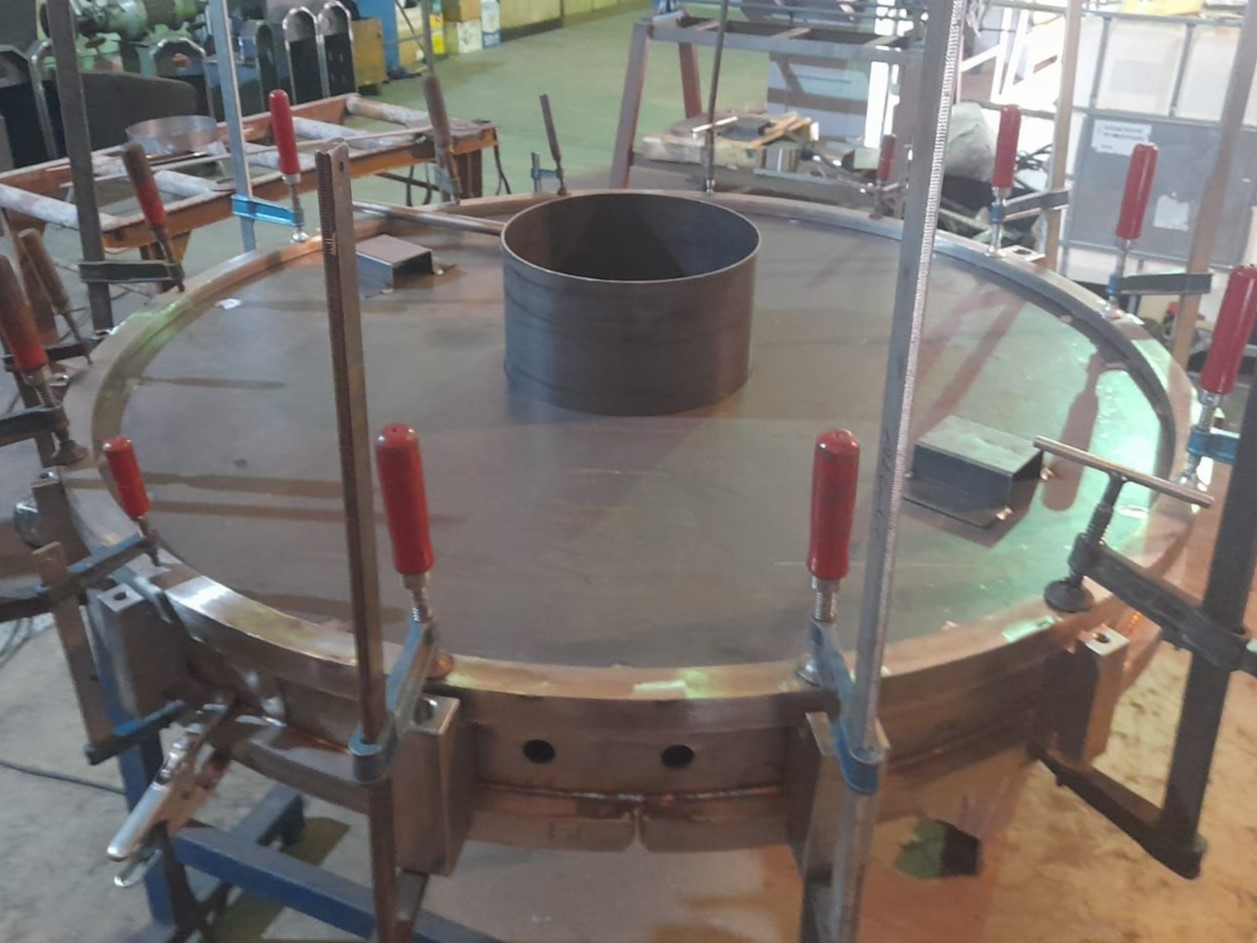
\includegraphics[width=.7\linewidth]{../../../figures/manif/toroidal_sheets/rhodo_middle_only_cropped.jpeg}
    \vspace{0pt}
    \caption{Middle part of the cavity containing the beam line.}
\end{figure}

\iffalse \begin{figure}
    %\captionsetup[subfigure]{justification=centering}
    %\captionsetup{justification=centering}
    \centering
    \begin{subfigure}{.5\textwidth}
      \centering
      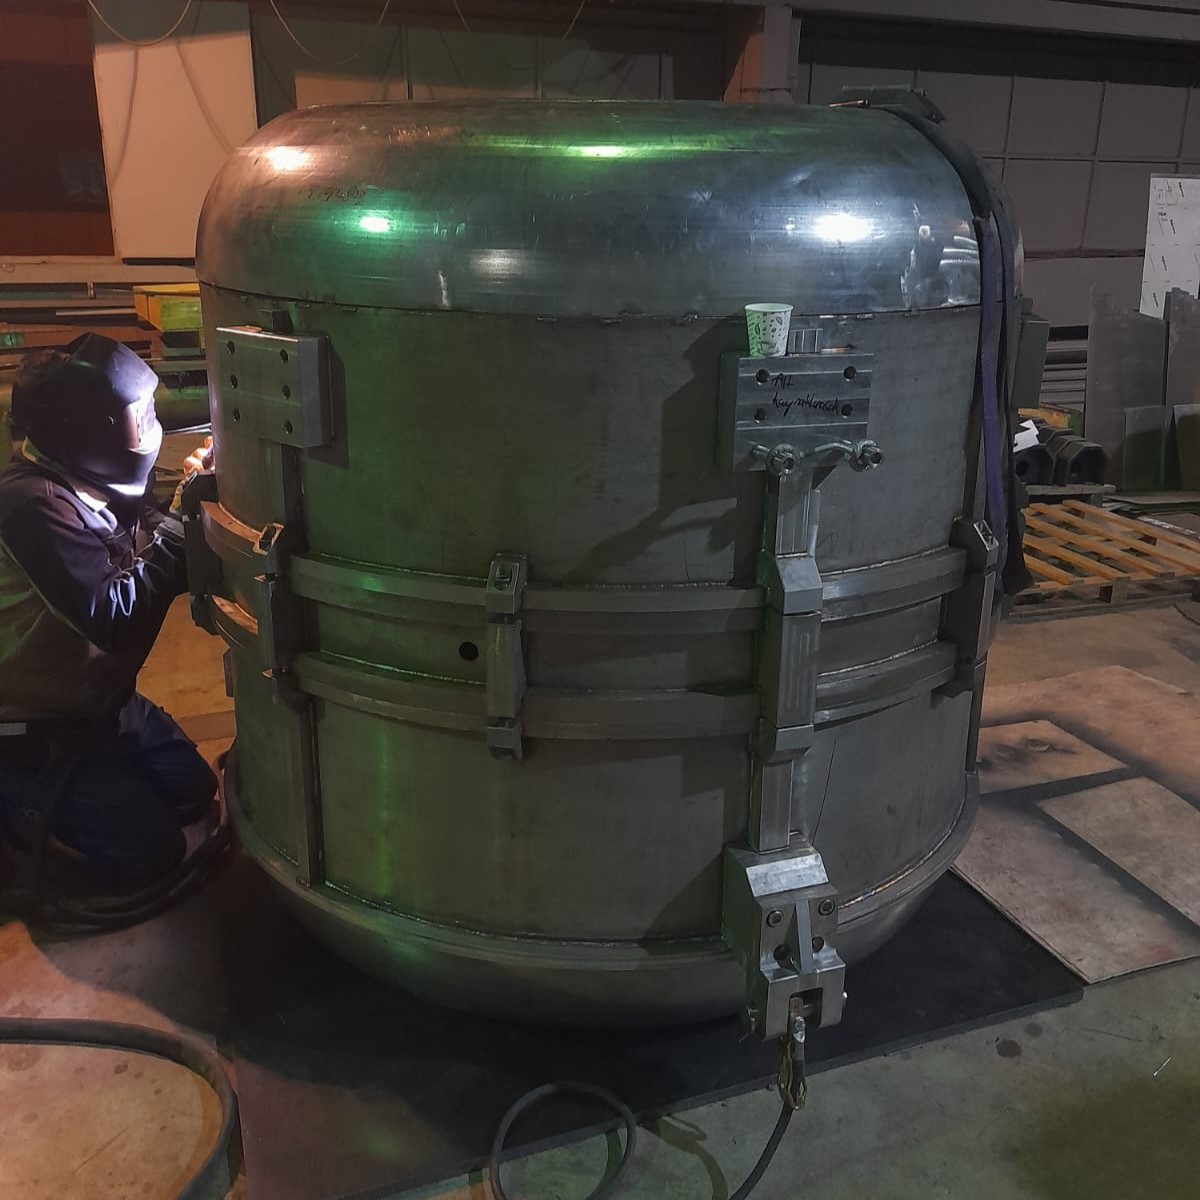
\includegraphics[width=.96\linewidth]{../../../figures/manif/welding/rhodo_assembled_welding_cropped.jpeg}
      \caption{Welding sheet bars.}
    \end{subfigure}%
    \centering
    \begin{subfigure}{.5\textwidth}
      \centering
      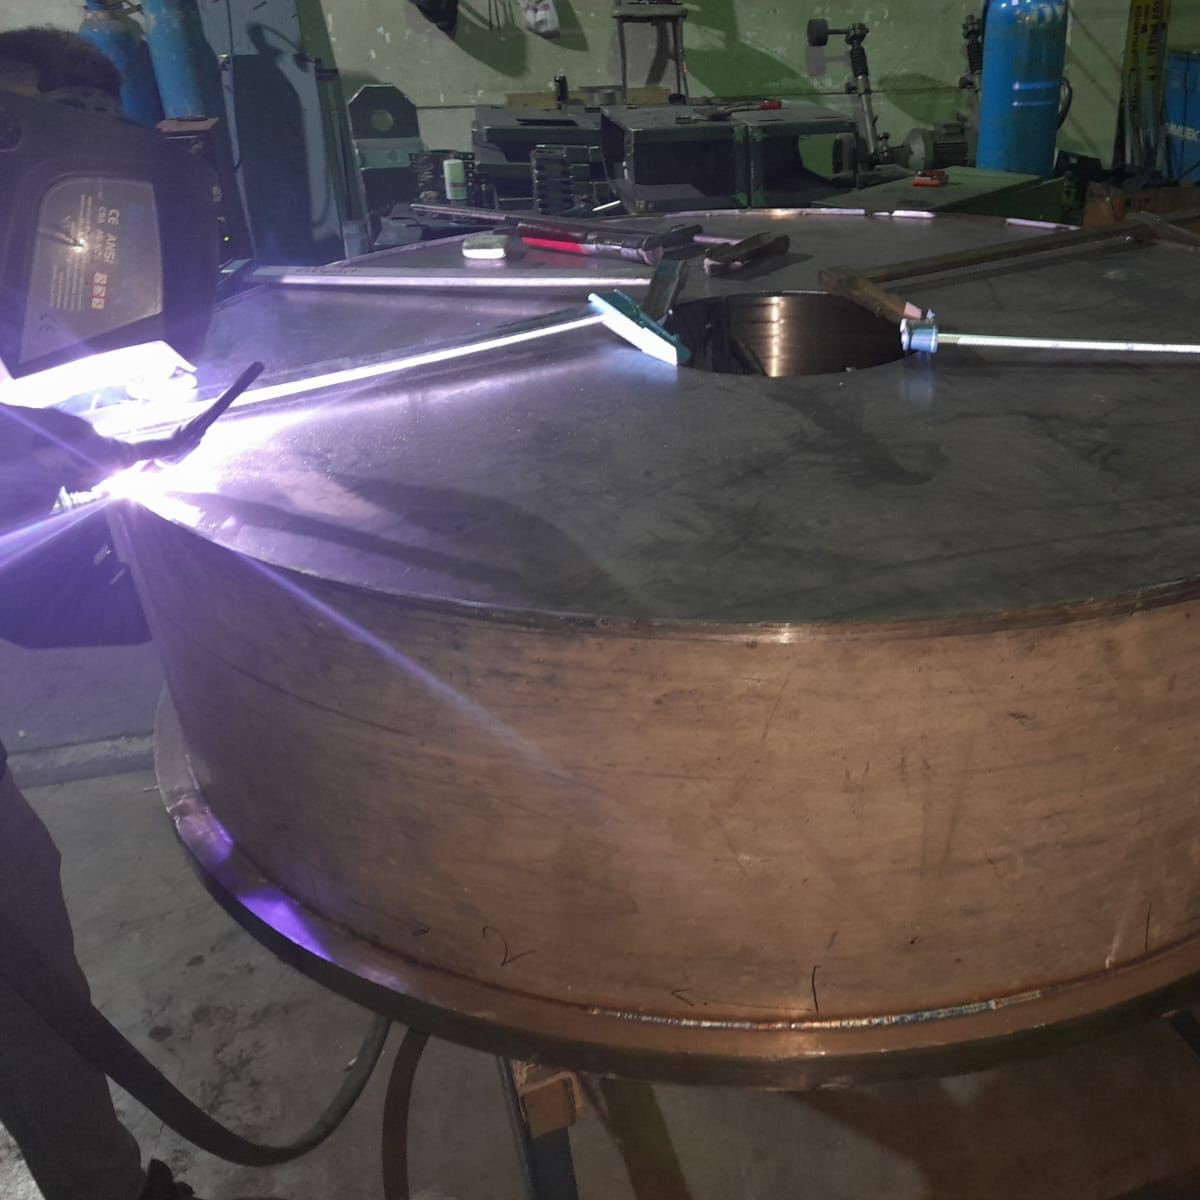
\includegraphics[width=.96\linewidth]{../../../figures/manif/welding/rhodo_middle_welding_toroidal_sheets_cropped.jpeg}
      \caption{Welding toroidal sheets.}
    \end{subfigure}
    \caption{TIG welding.}
    \label{fig:manif_welding}
\end{figure} \fi
\begin{figure}[H]
    \centering
    \subfigure[\centering Welding sheet bars]{{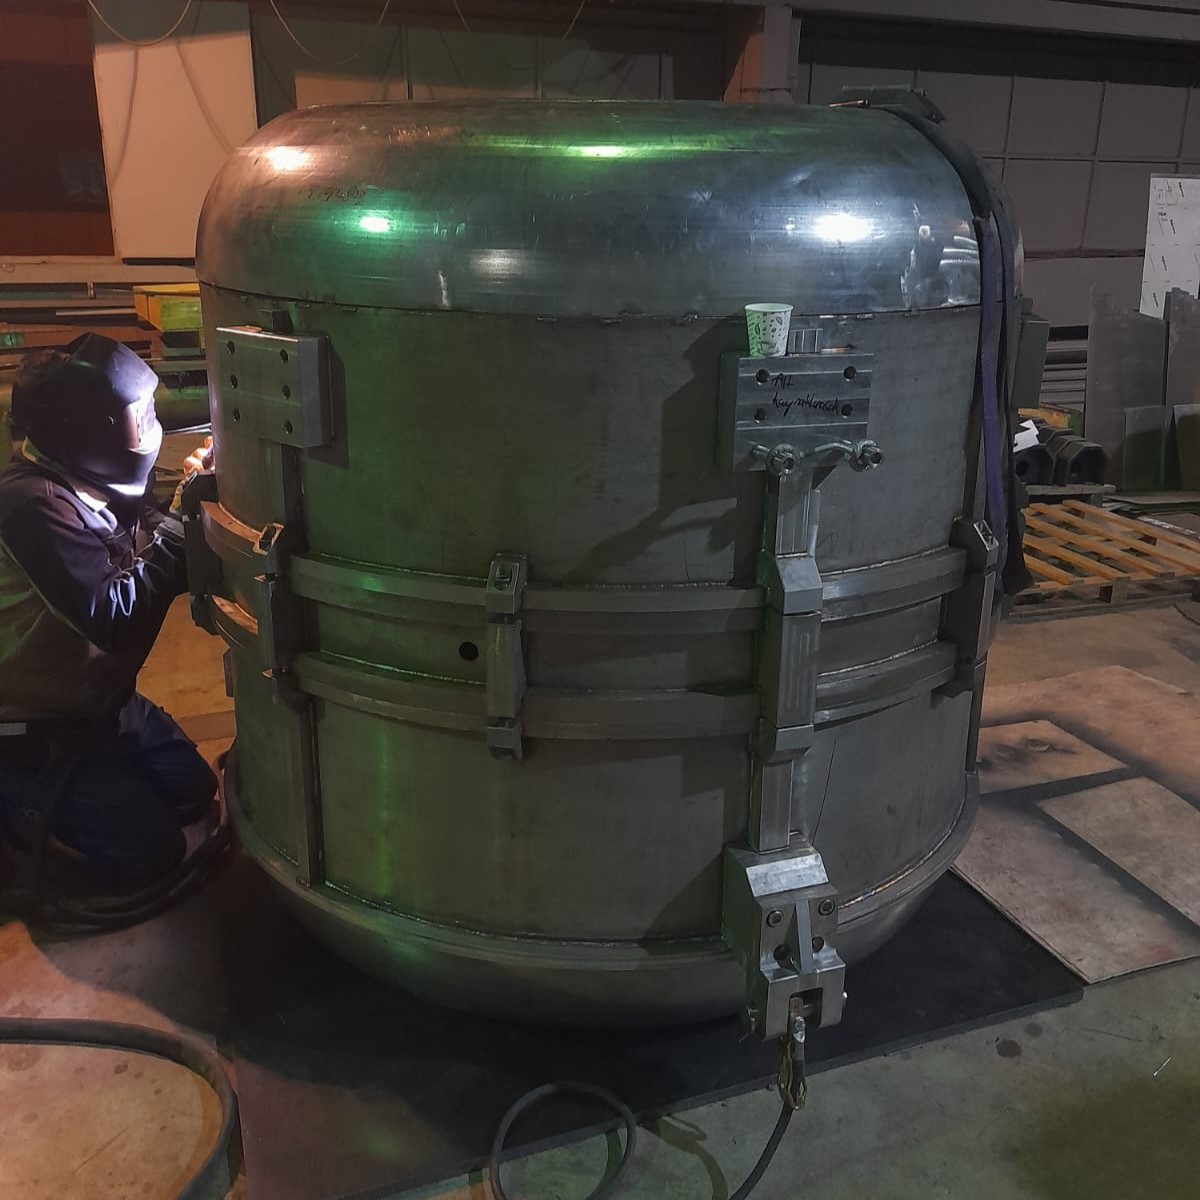
\includegraphics[width=.46\textwidth]{../../../figures/manif/welding/rhodo_assembled_welding_cropped.jpeg} }}%
    \qquad\subfigure[\centering Welding toroidal sheets]{{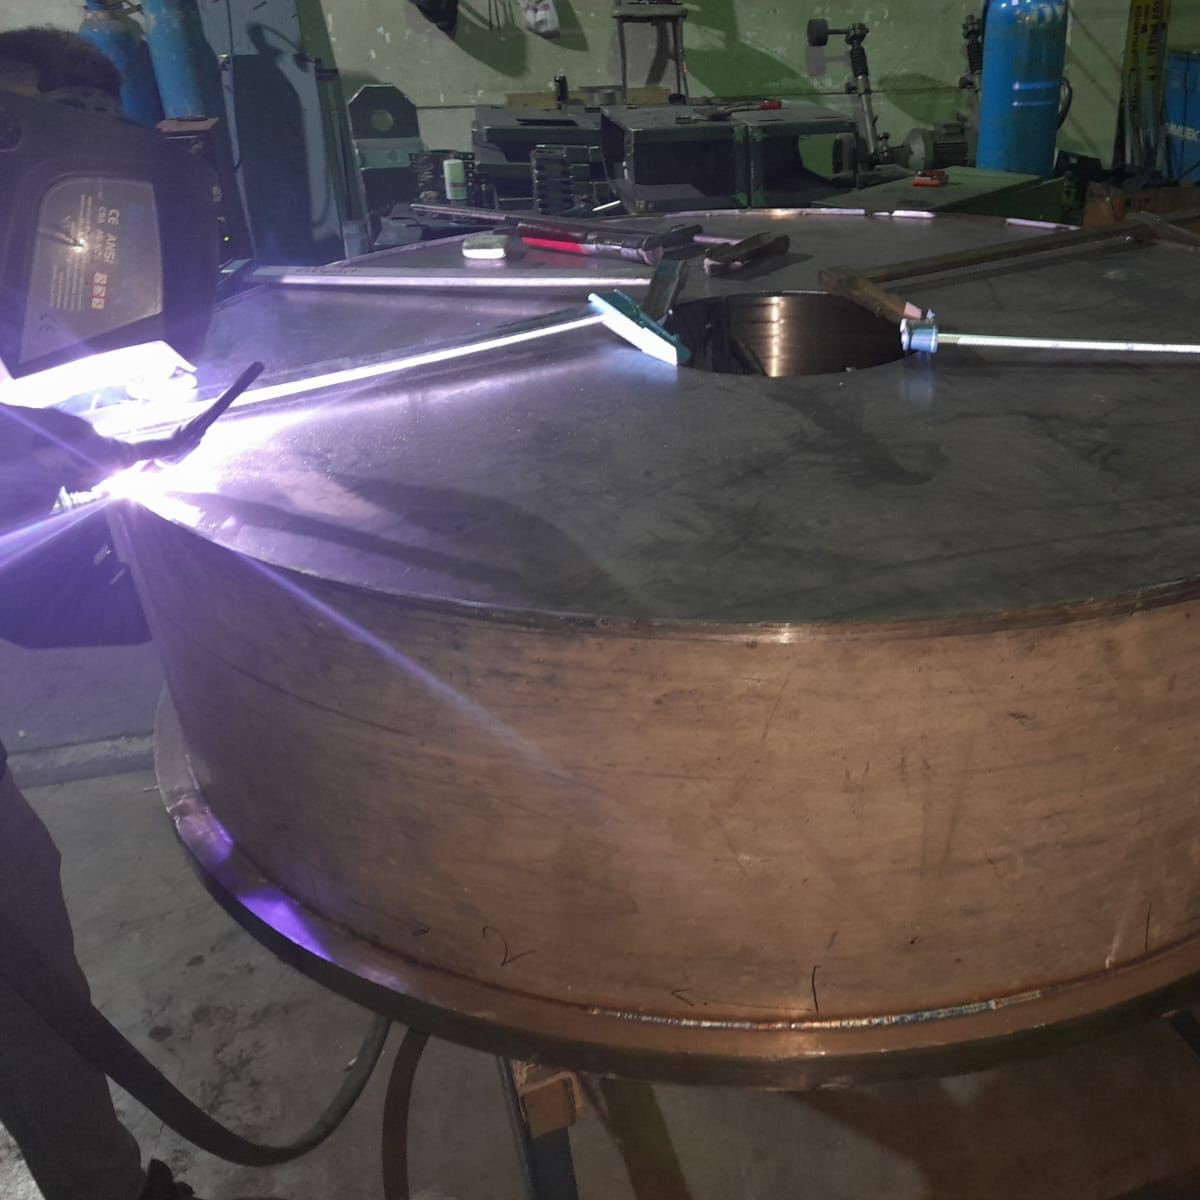
\includegraphics[width=.46\textwidth]{../../../figures/manif/welding/rhodo_middle_welding_toroidal_sheets_cropped.jpeg} }}%
    \vspace{5pt}
    \caption{\centering TIG welding.} 
    \label{fig:manif_welding}
    \vspace{5pt}
\end{figure}

\iffalse \begin{figure}
    %\captionsetup[subfigure]{justification=centering}
    %\captionsetup{justification=centering}
    \centering
    \begin{subfigure}{.5\textwidth}
      \centering
      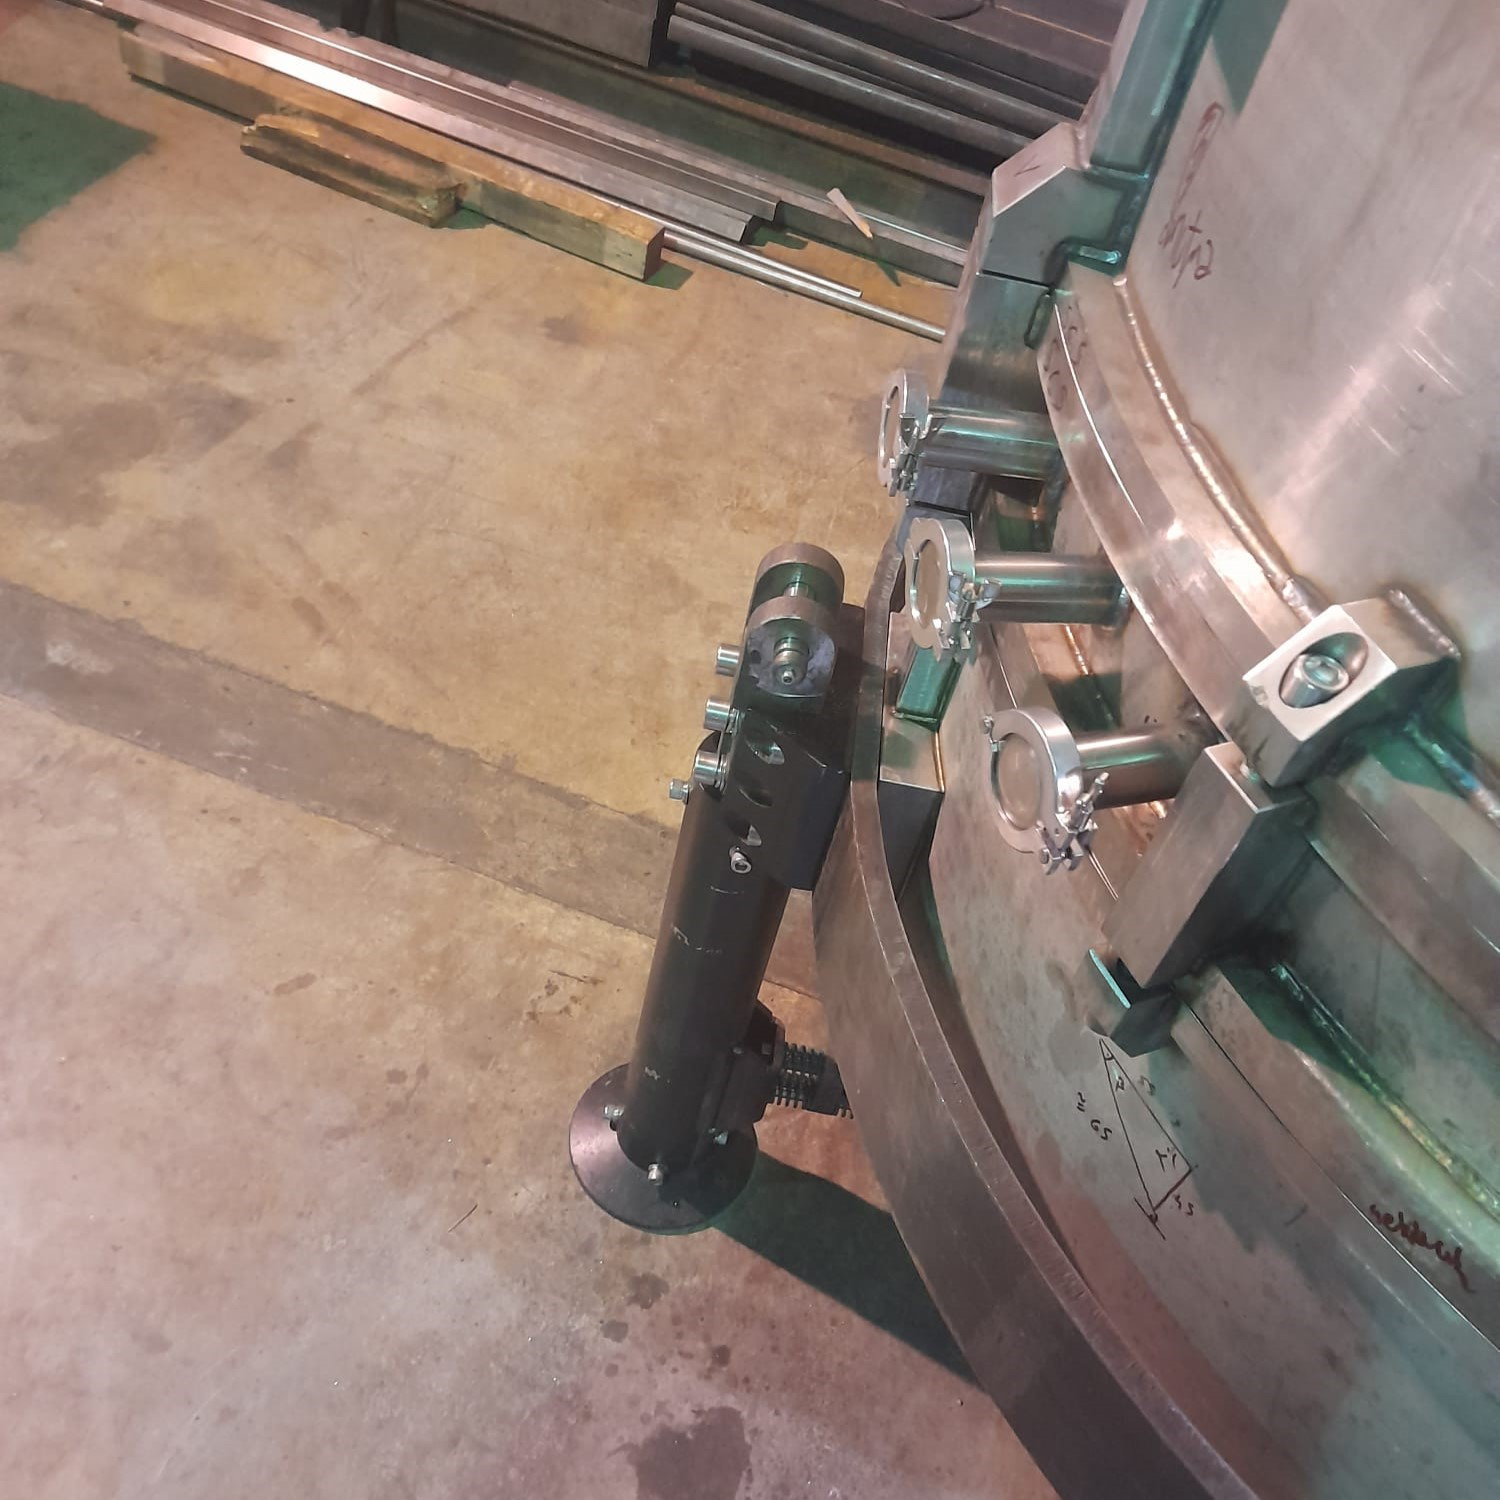
\includegraphics[width=.96\linewidth]{../../../figures/manif/assembled/rhodo_final_cropped_5.jpeg}
      \caption{Beam enter \& exit flanges.}
    \end{subfigure}%
    \centering
    \begin{subfigure}{.5\textwidth}
      \centering
      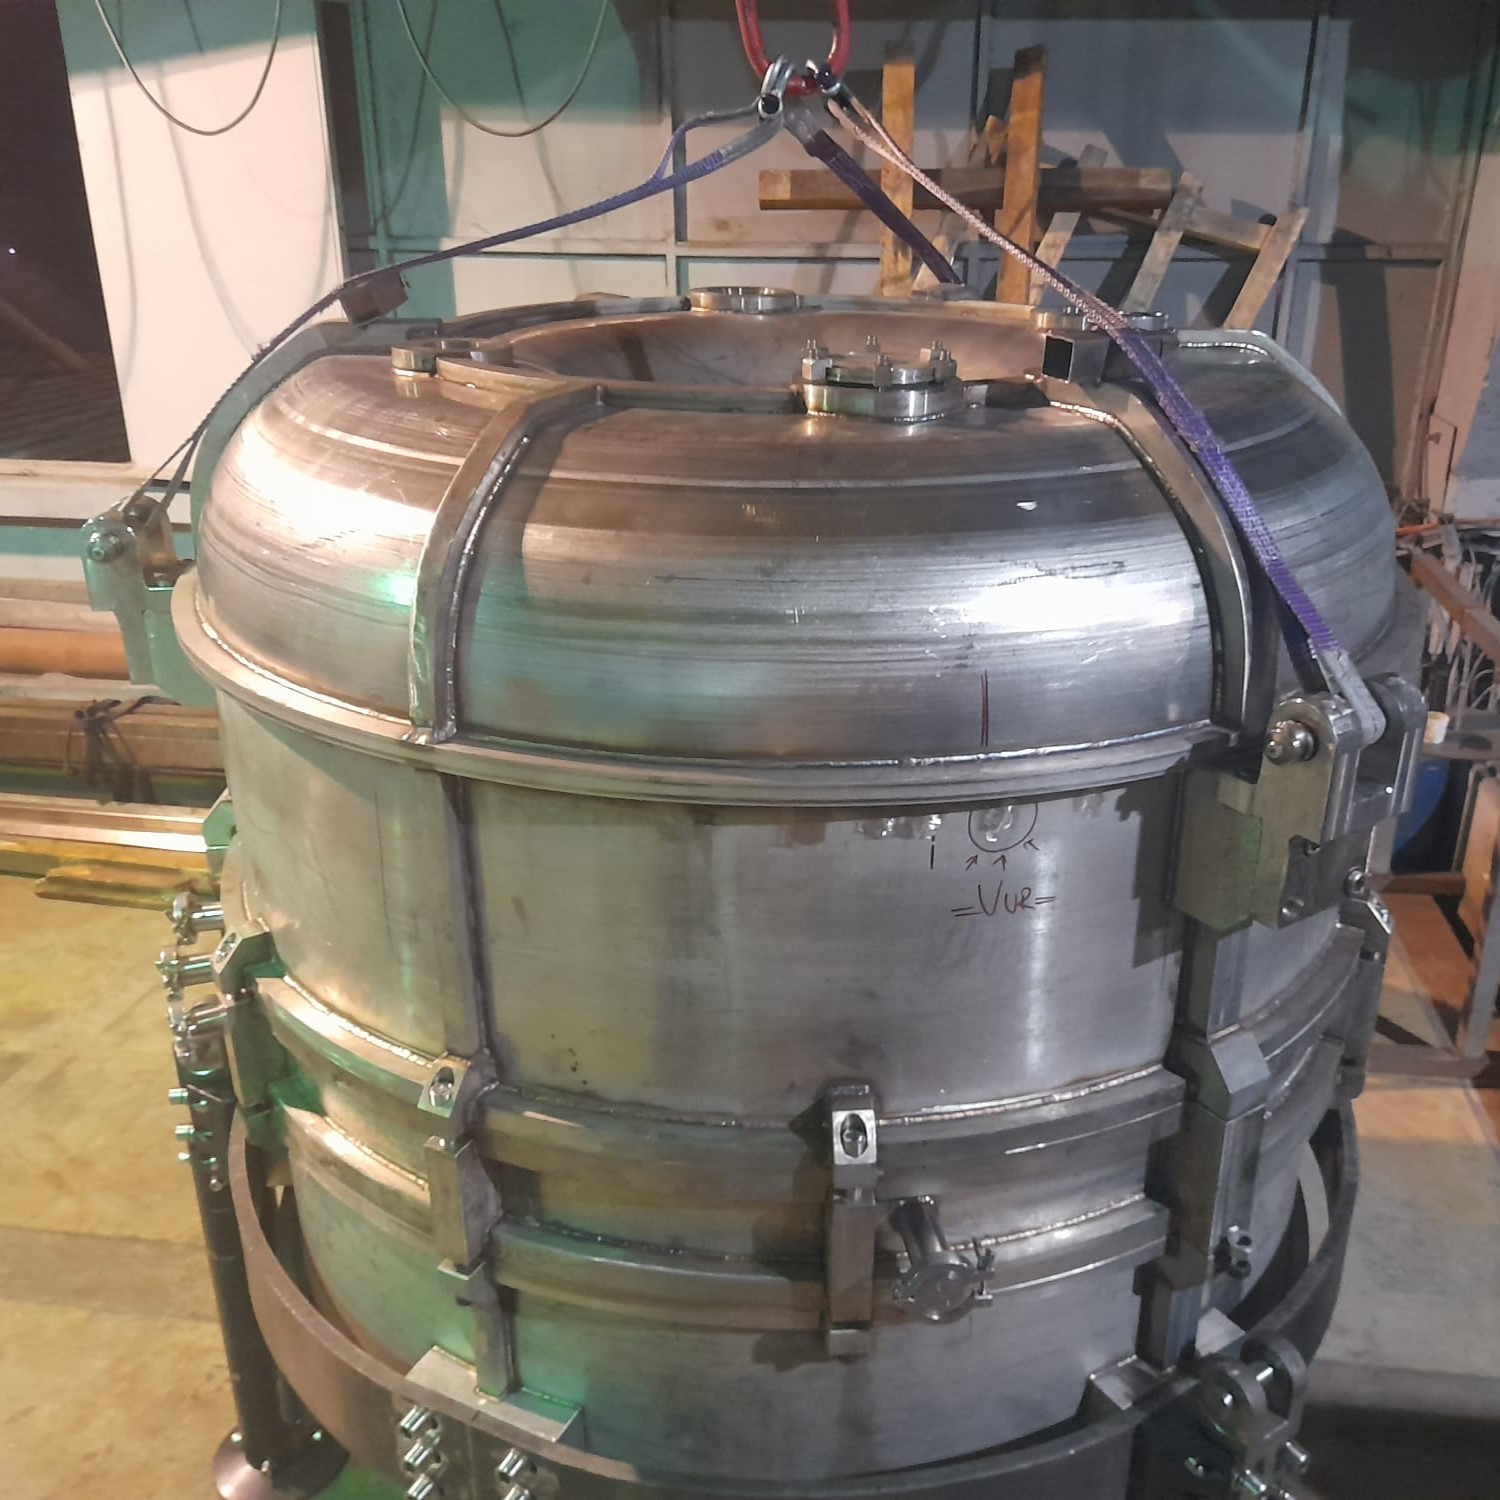
\includegraphics[width=.96\linewidth]{../../../figures/manif/assembled/rhodo_final_4_cropped.jpeg}
      \caption{RF input \& probe flanges.}
    \end{subfigure}
    \caption{Flanges on the assembled cavity.}
    \label{fig:manif_assembled_flanges}
\end{figure} \fi
\begin{figure}[H]
    \centering
    \subfigure[\centering Beam enter \& exit flanges]{{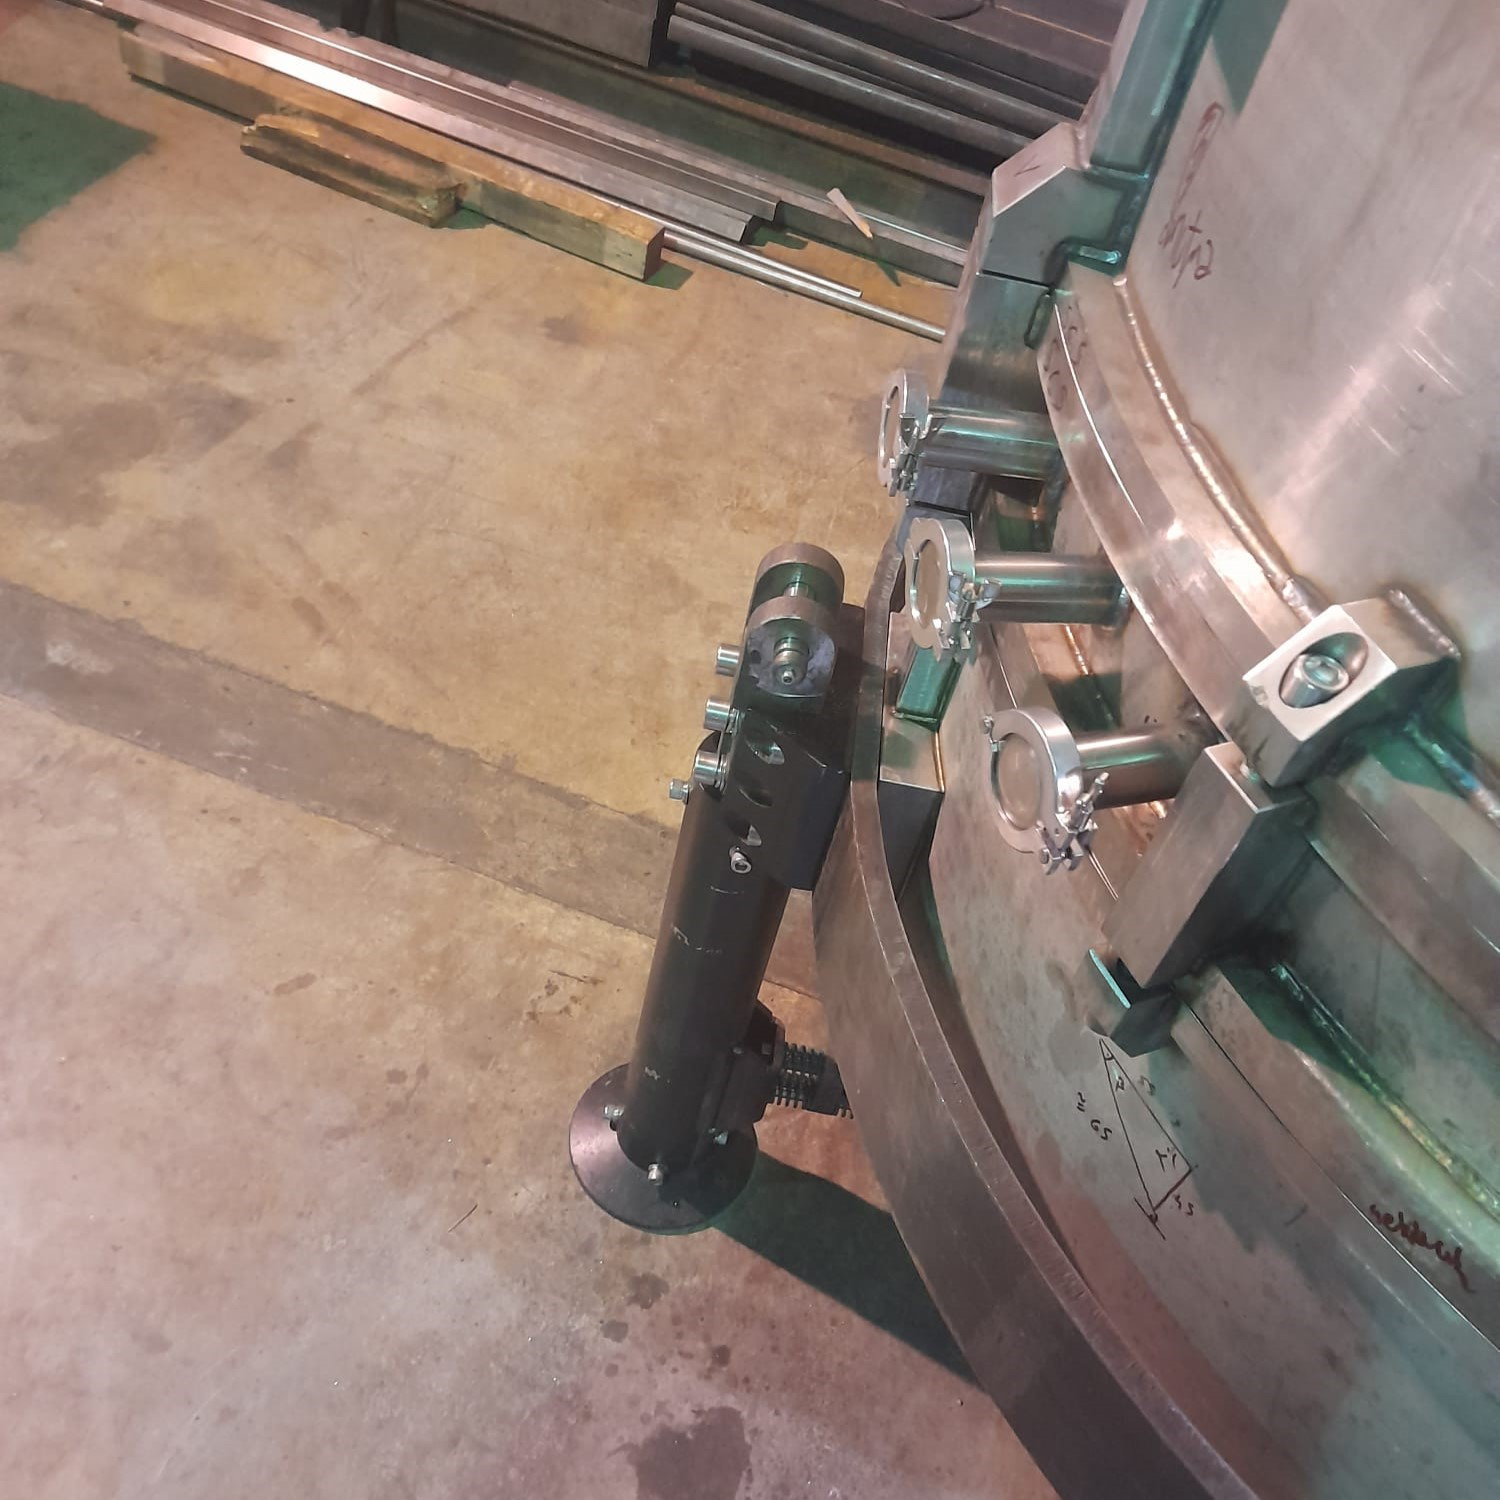
\includegraphics[width=.46\textwidth]{../../../figures/manif/assembled/rhodo_final_cropped_5.jpeg} }}%
    \qquad\subfigure[\centering RF input \& probe flanges]{{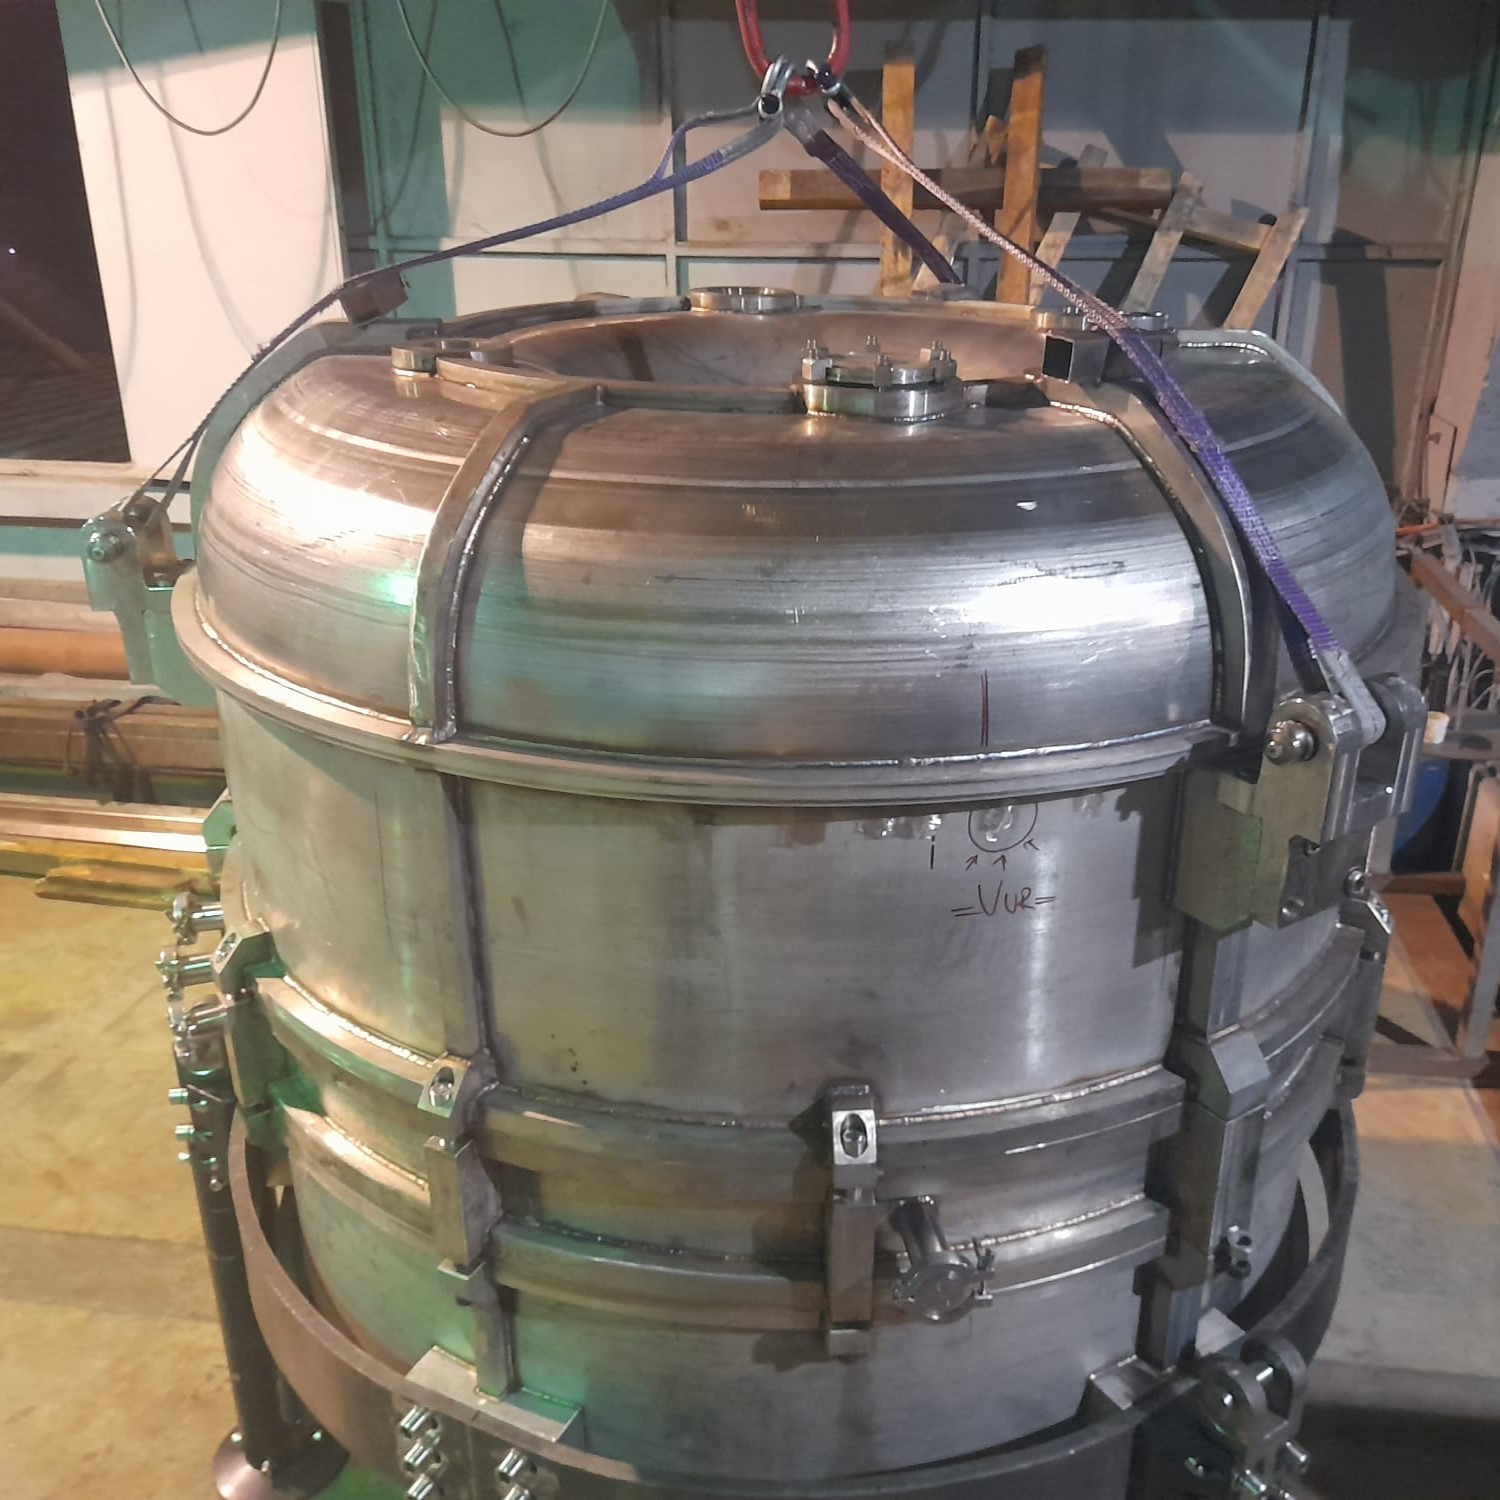
\includegraphics[width=.46\textwidth]{../../../figures/manif/assembled/rhodo_final_4_cropped.jpeg} }}%
    \vspace{5pt}
    \caption{\centering Flanges on the assembled cavity.} 
    \label{fig:manif_assembled_flanges}
\end{figure}

\begin{figure}[H]
    %%\captionsetup{justification=centering}
    \centering
    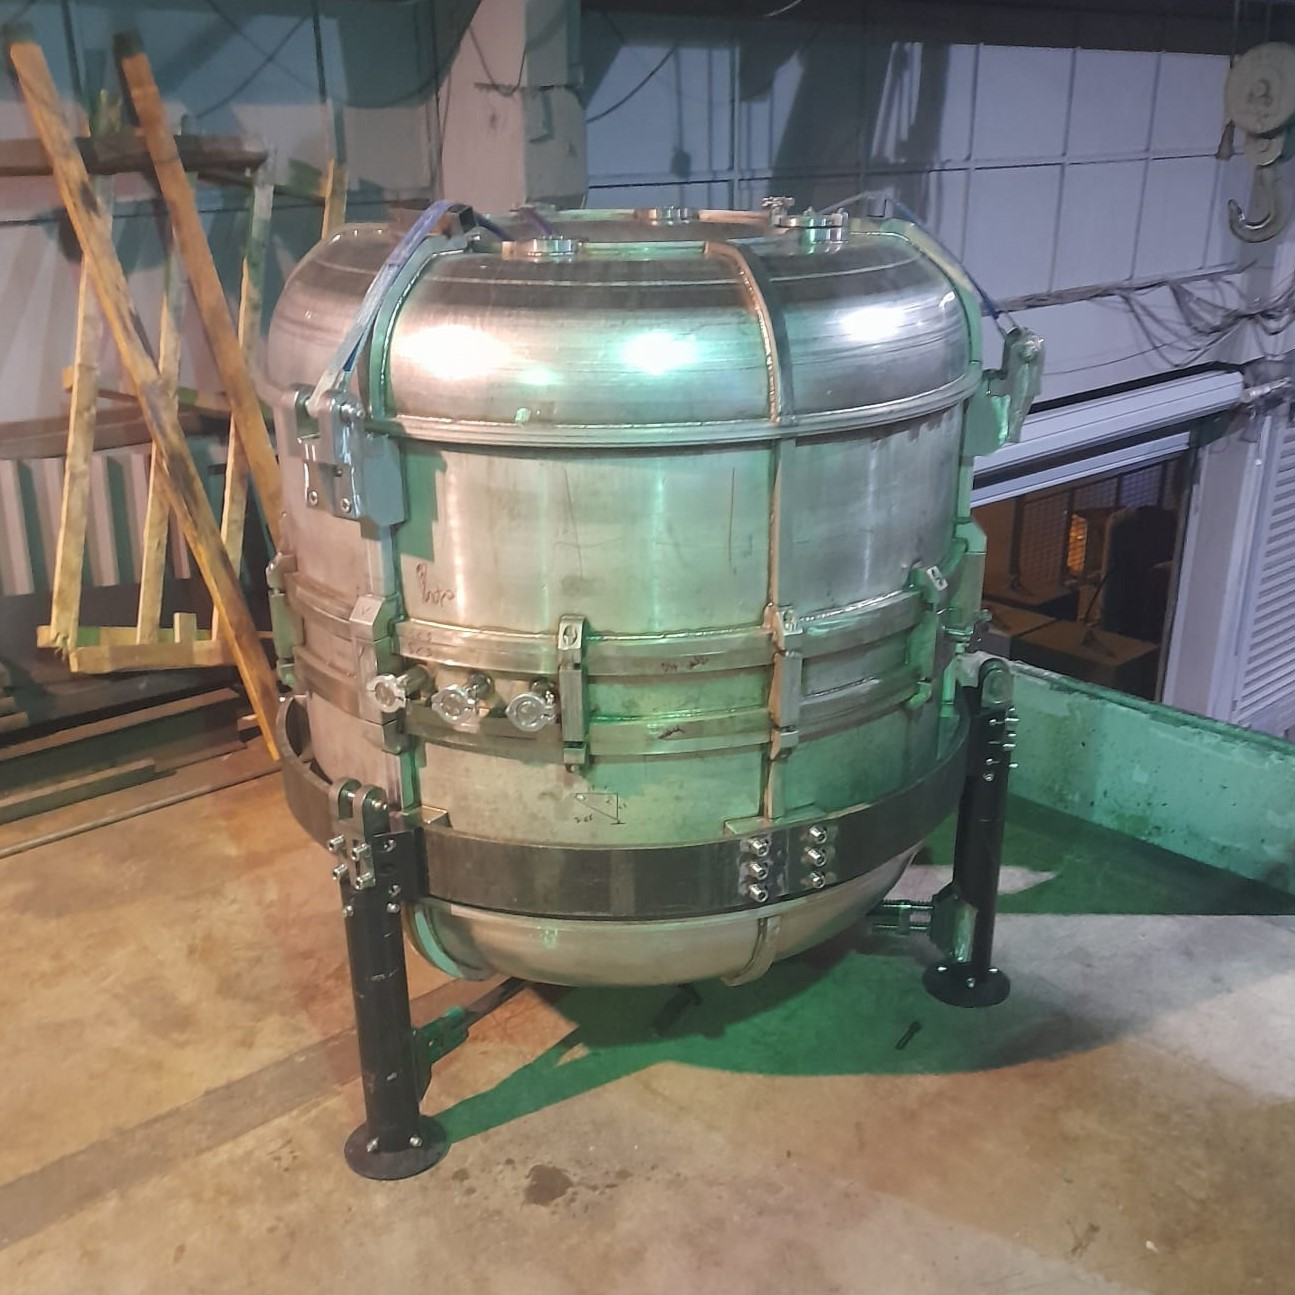
\includegraphics[width=.9\linewidth]{../../../figures/manif/assembled/rhodo_final_cropped.jpeg}
    \vspace{0pt}
    \caption{Current stage of the cavity.}
    \label{fig:manif_assembled}
\end{figure}


%%%%%%

\end{document}